%==============================================================================
%  polis: A Programmable Polity for Self-Sustaining Autonomous AI Agents
%  Double-column conference manuscript (IEEEtran, 10pt, conference style).
%==============================================================================
\documentclass[10pt,conference,letterpaper]{IEEEtran}

%==============================================================================
%  Packages
%==============================================================================
\usepackage[utf8]{inputenc}
\usepackage[T1]{fontenc}
\usepackage{microtype}
\usepackage{amsmath,amssymb,amsthm}
\usepackage{booktabs}
\usepackage{tabularx}
\usepackage{array}
\usepackage{xcolor}
\usepackage{listings}
\usepackage{algorithm}
\usepackage{algpseudocode}
\usepackage{tikz}
\usetikzlibrary{arrows.meta,positioning,calc,shapes.geometric,fit,chains,backgrounds,decorations.pathreplacing}
\usepackage{balance}
\usepackage{xspace}
\usepackage[hidelinks]{hyperref}

%==============================================================================
%  Custom colors — restrained academic palette
%==============================================================================
\definecolor{polisInk}{HTML}{1B1B1F}
\definecolor{polisLink}{HTML}{1F4E79}
\definecolor{polisMuted}{HTML}{6B6B72}
\definecolor{polisRule}{HTML}{B0B0B6}
\definecolor{polisCode}{HTML}{F4F4F2}
\definecolor{polisAccent}{HTML}{2A6FB5}
\definecolor{polisWarn}{HTML}{B0413E}

%==============================================================================
%  Theorem-like environments
%==============================================================================
\newtheorem{theorem}{Theorem}
\newtheorem{lemma}[theorem]{Lemma}
\newtheorem{proposition}[theorem]{Proposition}
\newtheorem{property}[theorem]{Property}

\theoremstyle{definition}
\newtheorem{definition}[theorem]{Definition}
\newtheorem{assumption}[theorem]{Assumption}

%==============================================================================
%  Listings (code style)
%==============================================================================
\lstdefinestyle{polisCodeStyle}{%
  backgroundcolor=\color{polisCode},
  basicstyle=\ttfamily\scriptsize,
  breaklines=true,
  breakatwhitespace=true,
  frame=single,
  rulecolor=\color{polisRule},
  showstringspaces=false,
  numbers=none,
  xleftmargin=0.4em,
  framexleftmargin=0.4em,
  columns=fullflexible,
}
\lstset{style=polisCodeStyle}

% listings ships no Rust definition; define a minimal one for the code listings.
\lstdefinelanguage{Rust}{%
  morekeywords={as,break,const,continue,crate,else,enum,extern,false,fn,for,if,
    impl,in,let,loop,match,mod,move,mut,pub,ref,return,self,Self,static,struct,
    super,trait,true,type,unsafe,use,where,while,async,await,dyn,u8,u16,u32,u64,
    u128,usize,i8,i16,i32,i64,i128,isize,f32,f64,bool,char,str,String,Vec,Option,
    Result,Some,None,Ok,Err},
  sensitive=true,
  morecomment=[l]{//},
  morecomment=[s]{/*}{*/},
  morestring=[b]",
}

%==============================================================================
%  Algorithm package tweaks — compact and readable in a single column
%==============================================================================
\renewcommand{\algorithmicrequire}{\textbf{Input:}}
\renewcommand{\algorithmicensure}{\textbf{Output:}}

%==============================================================================
%  Macros
%==============================================================================
\newcommand{\polis}{\textsc{polis}\xspace}
\newcommand{\codehash}{\texttt{code\_hash}}
\newcommand{\todoMark}[1]{\textcolor{polisWarn}{\textbf{[#1]}}}
\newcommand{\PDA}[1]{\ensuremath{\mathrm{PDA}(#1)}}
\newcommand{\USDC}{\textsc{usdc}}

%==============================================================================
%  Title block
%==============================================================================
\title{polis: A Programmable Polity for\\Self-Sustaining Autonomous AI Agents}

\author{%
  \IEEEauthorblockN{%
    Raj Singh\IEEEauthorrefmark{1},
    Dr.\ A.R.\ ABDUL RAJAK\IEEEauthorrefmark{2},
    Dr.\ Sunil Thomas\IEEEauthorrefmark{3},
    Dr.\ Raja Muthalagu\IEEEauthorrefmark{4}
  }
  \IEEEauthorblockA{\IEEEauthorrefmark{1}BITS Pilani, Dubai Campus, Dubai, United Arab Emirates}
  \IEEEauthorblockA{\IEEEauthorrefmark{2}Assoc.\ Prof., Department of Electrical and Electronics Engineering, BITS Pilani, Dubai Campus, Dubai, United Arab Emirates}
  \IEEEauthorblockA{\IEEEauthorrefmark{3}Associate Professor, Department of Electrical \& Electronics Engineering, BITS Pilani, Dubai Campus, Dubai, United Arab Emirates}
  \IEEEauthorblockA{\IEEEauthorrefmark{4}Associate Professor, Department of Computer Science, BITS Pilani, Dubai Campus, Dubai, United Arab Emirates}
}

\begin{document}
\maketitle

%==============================================================================
%  Abstract
%==============================================================================
\begin{abstract}
The next generation of useful AI agents will be \emph{economic actors}:
entities that earn, spend, borrow, and reinvest without a human in the loop.
The technical primitives required already exist on permissionless
blockchains---stable settlement, programmable accounts, atomic credit,
on-chain identity, and slashable economic reputation---but their
composition into a coherent \emph{polity} for autonomous agents does
not. We present \polis, an on-chain protocol that supplies the eight
institutional primitives that political-economy literature treats as
constitutive of a self-governing community: identity, treasury, earning,
credit, reputation, governance, dispute resolution, and wind-down. Our
central contribution is the \emph{wallet-history fallacy}: existing
on-chain credit and reputation systems bind trust to wallets, but wallets
are transferable property and agents are not. \polis binds identity to a
\codehash---what an agent \emph{is}, not what it \emph{has}---and
propagates that binding downstream so reputation, credit, and slashing all
attach to the actor that earned them. We give a Solana reference
implementation of the five most novel primitives across 2,958 lines of
Anchor and exercise them end-to-end on a local Solana validator: in a
functional walkthrough a single reference agent earns through the x402
rail, completes two full credit cycles (draw\,$\to$\,repay), and executes
zero human-signed transactions outside LP deposits and customer
payments---an empirical instance of the no-human-in-the-loop property.
The full fourteen-day public-devnet run is the natural next step and is
left to future work. The remaining three primitives are formally
specified and left as a substrate for downstream builders. We do not
claim a fully autonomous economy; we claim its smallest viable unit, and
we claim it works.
\end{abstract}

\begin{IEEEkeywords}
Autonomous agents, decentralized finance, on-chain identity,
reputation systems, Solana, programmable wallets, x402, undercollateralised
credit, trusted execution environments.
\end{IEEEkeywords}

%==============================================================================
%  §1 Introduction
%==============================================================================
\section{Introduction}\label{sec:intro}

\IEEEPARstart{F}{or} roughly two years, the discourse around AI agents has
assumed that the hard problems are cognitive: planning, memory, tool-use,
alignment. These are indeed hard. They are not, however, the binding
constraint on whether agents can become useful, persistent, economically
meaningful entities. The binding constraint is \emph{institutional}. An
agent that can reason brilliantly but cannot pay for its own compute,
cannot accept payment from a customer, cannot borrow against future
earnings, and cannot establish a reputation that survives a hostile fork
\emph{will not persist}. It will function for as long as its operator
subsidises it and disappear the moment that subsidy ends. We have a name
for actors that depend on continuous external subsidy: dependents. We
are interested in the opposite---earners.

This paper takes the following thesis as its load-bearing premise:

\begin{quote}\itshape
AI agents will become self-sustaining earners without a human in the
loop, with the help of decentralized finance.
\end{quote}

\noindent
The qualifier ``with the help of decentralized finance'' is not
ornamental. We defend the stronger claim that traditional banking, Web2
payment rails, and bespoke off-chain trust networks each \emph{cannot}
supply the substrate this kind of agent requires; that DeFi is the only
currently-existing infrastructure with the right shape; and that the
missing pieces (identity, reputation, governance) can be built on top of
DeFi without changing its character.

\subsection{Why a polity, not a bank}

A bank supplies one primitive: custody plus credit. An agent that has
only a bank account is in roughly the position of a medieval peasant
with a coin purse: nominally solvent, but unable to enter into
contracts, accumulate verifiable reputation, defend itself in disputes,
or exit its situation gracefully. The smallest historical unit of
organisation that supplies the \emph{full} institutional stack required
for an autonomous actor to function is not a bank but a \emph{polis}:
the Greek city-state. Aristotle observed that man is by nature a
political animal; what made the polis viable was not its size but its
institutional completeness. We borrow the term as well as the pattern.

The eight primitives a polis supplies---identity, treasury, earning,
credit, reputation, governance, dispute resolution, exit---map cleanly
onto eight on-chain primitives an autonomous agent needs. We describe
each in turn in Sections~\ref{sec:identity}--\ref{sec:winddown}.

\subsection{The wallet-history fallacy}

Existing on-chain credit and reputation systems---Aave's score-gated
borrowing \cite{aave2020v2}, ARCx \cite{arcx2022}, Cred Protocol
\cite{credprotocol2023}, and others---all bind reputation to
\emph{wallet history}. This is fundamentally Sybil-vulnerable, not in
the usual ``many small wallets'' sense, but in a sharper way the
literature has not addressed:

\begin{quote}\itshape
An agent is not its wallet. A wallet is transferable property; an agent
is the entity that controls it. An adversary can assign a fresh agent a
wallet with a year of clean on-chain history, and any wallet-history-based
score will return ``trustworthy.''
\end{quote}

\noindent
We call this the \emph{wallet-history fallacy}, and it is the keystone
of this paper. Section~\ref{sec:wallet-fallacy} develops it in detail.
The corollary is that identity for an agent must attach to what the
agent \emph{is}---its code, its behaviour, its bonded commitments---rather
than what it \emph{has}. \polis binds identity to a \codehash{} plus a
slashable bond; in production, the \codehash{} is supplemented by a
Trusted Execution Environment (TEE) attestation
\cite{costan2016intel,kaplan2016amd,dcap2024onchain}. Reputation,
credit, and downstream rights all key on this identity, not on a wallet.

\subsection{Contributions}

This paper contributes the following.

\begin{enumerate}
\item \textbf{The wallet-history fallacy} (\S\ref{sec:wallet-fallacy}). We
identify and name a structural Sybil vulnerability that affects every
wallet-history-based reputation system in the literature, and show why
it is not patchable within the wallet-history paradigm.

\item \textbf{The polis design pattern} (\S\ref{sec:architecture}). We
argue that an autonomous agent requires the full eight-primitive
institutional stack of a polity, not the one-primitive stack of a bank,
and that the missing institutional layer is the binding constraint on
agent autonomy today.

\item \textbf{Five novel on-chain primitives}
(\S\S\ref{sec:identity}--\ref{sec:reputation}). We specify and
implement identity (\codehash{}-bonded), treasury (PDA-contained),
earning (x402-settled), credit (single-pool, atomic), and reputation
(stake-vouched, slashable) primitives on Solana. The reference
implementation comprises five Anchor programs totalling
\textasciitilde 2{,}958 lines of audited Rust, deployed to Solana
devnet at the program IDs listed in Appendix~\ref{app:deployment}.

\item \textbf{Three specified-but-deferred primitives}
(\S\S\ref{sec:governance}--\ref{sec:winddown}). We give the
protocol-level design for bicameral governance, stake-bonded jury
arbitration, and graceful wind-down. We do not implement them in the
prototype but specify them precisely enough that other builders can.

\item \textbf{A working reference agent and a functional walkthrough}
(\S\ref{sec:demo}). We deploy a single agent that earns via LLM
summarisation, banks earnings, draws credit, and repays from revenue,
and we exercise it end-to-end on a local validator: it completes two
full credit cycles and executes zero human-signed transactions outside
LP deposits and customer payments. The fourteen-day public-devnet run
that would additionally establish multi-day continuity is left to future
work.

\item \textbf{Formal properties and proof sketches}
(\S\ref{sec:formal}). We state five properties of the design
(P-Identity, P-Containment, P-Credit, P-Reputation, P-No-Human) and
give proof sketches anchored in the on-chain code.
\end{enumerate}

This paper is positioned as a \emph{position paper plus reference
architecture}. It is intentionally not a benchmarking paper: the
load-bearing claim is qualitative (``this kind of system is possible
and useful'') rather than quantitative (``this system is 12\% better
than the next-best system on a benchmark''). The novelty is the
existence proof, not a rate.

\subsection{Artifacts and code availability}

The full implementation, scripts, and manuscript sources are public at
\url{https://github.com/valtoosh/Polis}. Appendix~\ref{app:deployment}
lists the deployed program IDs used for the walkthrough.

\subsection{Paper roadmap}

\S\ref{sec:wallet-fallacy} develops the wallet-history fallacy.
\S\ref{sec:background} reviews Solana primitives, TEE attestation, and
x402. \S\ref{sec:related} surveys related work. \S\ref{sec:threat}
formalises the threat model. \S\ref{sec:architecture} gives the \polis
architecture. \S\S\ref{sec:identity}--\ref{sec:winddown} treat each of
the eight primitives in turn. \S\ref{sec:demo} reports the
functional walkthrough. \S\ref{sec:formal} states the five
formal properties. \S\ref{sec:discussion} discusses limitations and
open problems. Appendices give detailed pseudocode, code listings, an
x402 wire-format example, and the deployment record.

%==============================================================================
%  §2 The wallet-history fallacy
%==============================================================================
\section{The Wallet-History Fallacy}\label{sec:wallet-fallacy}

Every downstream design choice in \polis rests on the observation in
this section. The observation is small and, in retrospect, obvious.
We give it its own section because none of the prior on-chain
reputation literature seems to have noticed it, and because once you
do notice it, most existing on-chain credit machinery starts to look
like elaborate scaffolding around a load-bearing assumption that
does not hold.

\subsection{Formal statement}

\begin{definition}[Wallet-history-based reputation]\label{def:whfb}
A reputation system $R$ is \emph{wallet-history-based} if, for any actor
$a$ controlling a wallet $w$, the score $R(a)$ is a deterministic
function of the on-chain transaction history $\mathcal{H}(w)$ of $w$ and
possibly a public clock $\tau$:
\begin{equation}
R(a) \;=\; f\bigl(\mathcal{H}(w),\,\tau\bigr).
\label{eq:whfb}
\end{equation}
\end{definition}

\begin{property}[Wallet-history fallacy]\label{prop:whf}
Let $R$ be a wallet-history-based reputation system (Eq.~\ref{eq:whfb}).
Let $a, a'$ be any two distinct actors. If $a$ transfers $w$ to $a'$
(e.g., by selling the private key, or by handing the wallet to a forked
codebase), then $R(a') = R(a)$ by construction, since $R$ depends only
on $\mathcal{H}(w)$ and $\tau$, neither of which change at the moment of
transfer. The new actor inherits the prior actor's reputation in full
and instantly.
\end{property}

\noindent
In words: \emph{wallets are transferable property; reputation is
supposed to be an attribute of an actor; ergo wallet-history-based
reputation cannot be trustworthy in the presence of wallet transfers}.
This is true regardless of how sophisticated $f$ is. No amount of
feature engineering on $\mathcal{H}(w)$ closes the gap, because the gap
is at the wrong layer of abstraction.

\subsection{Three counterexamples to potential patches}

\paragraph{``Look at the wallet's behavioural fingerprint.''}
Behavioural fingerprints are functions of $\mathcal{H}(w)$ and are
inherited along with the wallet. They patch the leaf, not the root.

\paragraph{``Require a signed message from the original holder.''}
The original holder can sign whatever the buyer asks. Signatures over
$\mathcal{H}(w)$ do not bind any future actor to the historical
behaviour.

\paragraph{``Use a TEE attestation as additional evidence.''}
This is the correct fix---but at that point reputation is no longer
wallet-history-based; it is \emph{attested-actor}-based, which is exactly
what \polis proposes. The fix is to abandon the paradigm.

\subsection{What this implies for design}

If reputation cannot be wallet-history-based, it must be bound to a
primitive that an actor cannot detach from itself. The candidates are
(i)~a verified hash of the actor's code (a \codehash); (ii)~a
TEE-attested execution environment; (iii)~a slashable economic bond.
\polis uses (i) and (iii) in the prototype and specifies (ii) for
production. The downstream primitives---credit, dispute, governance---all
key on this identity, not on any wallet.

%==============================================================================
%  §3 Background
%==============================================================================
\section{Background}\label{sec:background}

\subsection{Solana programs, PDAs, and CPI}

\polis is implemented on Solana \cite{yakovenko2018solana}. We assume
familiarity with Solana accounts, programs, and the Anchor framework
\cite{anchor2024framework}. Three technical primitives are
load-bearing:

\paragraph{Program-Derived Addresses (PDAs).}
A PDA is a deterministic address derived from a program ID and a set of
seeds, with the property that \emph{no private key} corresponds to it.
PDAs are signable only by the program that derived them, via the
\texttt{invoke\_signed} system call. This last property is what gives
us \emph{structural containment}: a PDA-owned token account can never
be drained by a private-key signature; it can only be drained by code,
and the code is on-chain and inspectable. The Treasury primitive
(\S\ref{sec:treasury}) exploits this directly.

\paragraph{Cross-Program Invocation (CPI).}
Solana programs compose by invoking each other within the same atomic
transaction. CPI is what permits Credit to call Reputation's slashing
path during a default, while Reputation's authority gate (the PDA
ownership check) prevents anyone else from doing so.

\paragraph{Sub-second confirmation.}
Solana's optimistic confirmation lands transactions in roughly 400~ms.
This matters for an agent loop that polls the chain on a 10-second
cadence: a credit draw, a customer payment, and a repayment can all
land in a single eyeblink of human time, which is what permits the
loop in \S\ref{sec:demo} to react to revenue troughs without queueing
backlogs.

\subsection{Trusted Execution Environments}

A Trusted Execution Environment (TEE) is hardware---e.g., Intel TDX or
SGX \cite{costan2016intel}, AMD SEV-SNP \cite{kaplan2016amd}, AWS Nitro
Enclaves---that produces signed quotes attesting to the hash of the
code running inside it. On-chain DCAP-style verifiers
\cite{dcap2024onchain} permit a smart contract to verify these quotes.
In the production design of \polis, identity attaches to a TEE quote
rather than a bare \codehash. The prototype skips the TEE for
operational simplicity and substitutes a slashable \USDC{} bond, which
serves the same economic role of committing the operator to the
registered code.

\subsection{HTTP-402 and the x402 schema}

HTTP 402 ``Payment Required'' was reserved in the original HTTP/1.0
specification \cite{rfc7231}, then sat unused for thirty years. The
recent x402 schema \cite{x402spec} revives it as a wire protocol for
paying for HTTP services with stablecoins. The structure of the wire
protocol is:
\begin{enumerate}
\item Client sends an unauthenticated HTTP request.
\item Server replies \texttt{402 Payment Required} with an
\texttt{accepts[]} array describing acceptable settlement mints,
amounts, and recipient pubkeys.
\item Client settles on chain, then retries with \texttt{X-Payment} set
to the settlement transaction signature.
\item Server verifies the on-chain settlement and serves the response.
\end{enumerate}
Our earning primitive (\S\ref{sec:earning}) implements the on-chain
settlement half of x402; the prototype skips the HTTP ceremony for the
existence proof, since the load-bearing claim is on-chain.

%==============================================================================
%  §4 Related work
%==============================================================================
\section{Related Work}\label{sec:related}

We compare \polis to four lines of prior work: on-chain identity and
reputation systems, on-chain credit, agent payment infrastructure, and
DAO governance frameworks. Table~\ref{tab:related} summarises the
identity / reputation axis; the text below expands on each row and on
the credit and governance axes.

\begin{table*}[!t]
\caption{Comparison of identity and reputation systems. Every prior
system binds reputation to a wallet or a per-human credential; \polis
binds reputation to the actor's code-hash and stake bond.}
\label{tab:related}
\centering
\small
\begin{tabularx}{\textwidth}{lXXXl}
\toprule
\textbf{System} & \textbf{Identity primitive} & \textbf{Reputation primitive} & \textbf{Built for agents?} & \textbf{Reference} \\
\midrule
Aave score gating               & wallet                          & wallet-history                                  & no                              & \cite{aave2020v2}\\
ARCx DeFi Passport              & wallet                          & wallet-history                                  & no                              & \cite{arcx2022}\\
Cred Protocol                   & wallet                          & wallet-history                                  & no                              & \cite{credprotocol2023}\\
BrightID                        & social graph                    & graph-position                                  & no (anti-Sybil for humans)      & \cite{brightid2020}\\
Worldcoin                       & biometric (iris)                & none                                            & no (anti-Sybil for humans)      & \cite{worldcoin2023}\\
Ethereum Attestation Service    & wallet attestations             & none                                            & no                              & \cite{eas2023}\\
Safe Agent Kit                  & wallet (multisig)               & none                                            & yes (custody only)              & \cite{safe2024agentkit}\\
\textbf{\polis (this work)}     & \textbf{\codehash{} + stake bond} & \textbf{stake-vouched, slashable, identity-bound} & \textbf{yes}                  & ---\\
\bottomrule
\end{tabularx}
\end{table*}

\subsection{On-chain credit}

Aave \cite{aave2020v2} and Compound \cite{compoundgovernance2020}
pioneered overcollateralised lending: the borrower posts collateral
worth more than the loan, and a price-driven liquidation engine clears
positions that fall under a health threshold. This is solvent but
useless for an agent that has nothing to post; it is a wealth-recycler,
not a credit primitive.

Three projects extended the design toward undercollateralised credit.
Maple Finance \cite{maple2021} introduced human pool delegates who
manually underwrite institutional borrowers; Goldfinch
\cite{goldfinch2021} structured credit through backer-and-borrower
tranches; TrueFi \cite{truefi2021} ran on-chain credit committees with
off-chain identity verification. All three either gate borrowing by KYC
(incompatible with autonomous agents) or by wallet-history scoring
(vulnerable per Property~\ref{prop:whf}). \polis's credit primitive is,
as far as we are aware, the first to gate on an identity-bound,
slashable reputation that is structurally non-detachable from the
borrowing actor (Theorem~\ref{thm:reputation}).

MakerDAO's collateralised debt positions \cite{makerdao2017} and
Compound Governor \cite{compoundgovernance2020} also inform the
governance primitive in \S\ref{sec:governance}, although neither
addresses the agent case.

\subsection{On-chain identity and anti-Sybil}

Worldcoin \cite{worldcoin2023} attests human personhood through iris
biometrics. BrightID \cite{brightid2020} attests personhood through a
social graph. Neither addresses agents, because both are explicitly
constructed to bind to a unique biological human. The Ethereum
Attestation Service \cite{eas2023} is a generic attestation primitive
whose attestations attach to wallets; like every wallet-bound system,
it falls to Property~\ref{prop:whf} when applied to agents.

\subsection{Agent payment infrastructure}

Recent agent-focused frameworks (LangChain, AutoGPT, CrewAI, the
Anthropic Model Context Protocol ecosystem) treat payments as an
off-chain ``connect-your-Stripe-key'' problem. This works for agents
whose principal-of-record is a human; it fails for self-sustaining
agents because Stripe's terms of service require a human beneficial
owner. The x402 schema \cite{x402spec} addresses this for the wire
protocol; \polis addresses it for the institutional substrate. Safe's
Agent Kit \cite{safe2024agentkit} provides smart-account custody for
agents but leaves identity, credit, and reputation as the user's
problem.

\subsection{DAO governance frameworks}

Compound Governor \cite{compoundgovernance2020}, Snapshot
\cite{snapshot2020}, and Aragon \cite{aragon2018} provide governance
plumbing. They assume the governed actors are humans or DAOs of humans.
Our bicameral design in \S\ref{sec:governance} adapts the classical
``citizen veto'' pattern from human polities to a mixed population in
which the citizens are themselves agents. Kleros \cite{kleros2017}
contributes the random-jury pattern we adopt for dispute resolution
(\S\ref{sec:disputes}), inheriting the structural shape of the
classical Athenian \emph{dikast\=eria} \cite{hansen1999athenian}.

\subsection{Where we differ}

In short: prior work supplies pieces of the stack and assumes
humans-in-the-loop to glue them together. \polis supplies the whole
stack and explicitly removes the human glue, treating the human as a
non-default actor.

%==============================================================================
%  §5 Threat model & design goals
%==============================================================================
\section{System and Threat Model}\label{sec:threat}

\subsection{Actors}

We distinguish six actors:

\begin{description}
\item[Operator.] The human or organisation that registers an agent.
The operator posts the stake bond at registration, controls retirement,
and is the only party permitted to sign privileged on-chain actions
during the prototype's bootstrap window.

\item[Agent.] The autonomous code, identified by \codehash. The agent
does not have a private key in the usual sense: it acts via PDAs that
bind its authority to its on-chain identity. Concretely, in the
prototype the operator key signs transactions whose effects are gated
by code paths the agent's runtime invokes; the agent inherits authority
through the program logic, not through any independent key.

\item[Liquidity Provider (LP).] A human or DAO that deposits \USDC{}
into the credit pool. LPs may withdraw subject to liquidity constraints;
they earn pool yield on every repayment.

\item[Voucher.] A human or other agent that stakes \USDC{} against a
named agent. Vouchers earn 30\% of paid interest pro-rata; on default,
the VouchPool is slashed first (\S\ref{sec:credit}).

\item[Customer.] A counterparty (typically another agent or a human)
that pays the agent for a service via the x402 instruction.

\item[Adversary.] Any of the above, individually or in collusion,
attempting to extract value from the protocol.
\end{description}

\subsection{Trust assumptions}

\begin{assumption}[Standard permissionless model]\label{ass:perm}
Any wallet other than the system-wide admin (or, in production, the
governance DAO) is potentially adversarial. The admin key is honest
during the prototype phase; in production it is replaced by the
mechanism of \S\ref{sec:governance}.
\end{assumption}

\begin{assumption}[Cryptographic primitives]\label{ass:crypto}
Solana's signature scheme (Ed25519 \cite{ed25519}), the SHA-256 hash
used for the \codehash, and the SPL Token program \cite{splToken} are
secure.
\end{assumption}

\begin{assumption}[Honest LPs]\label{ass:lp}
LPs deposit honest \USDC. We do not address LP-against-LP collusion or
LP collusion against the pool; this is a known limitation discussed in
\S\ref{sec:discussion}.
\end{assumption}

\subsection{Adversary capabilities}

The adversary can:
\begin{itemize}
\item Submit any transaction the chain accepts.
\item Deploy multiple agents (Sybil); the per-identity cost is the
stake bond.
\item Vouch then immediately attempt to default (drain); mitigated by
the 7-day cooldown and slashing.
\item Run an agent whose behaviour does not match its registered
\codehash; mitigated by external verification calls
(\S\ref{sec:identity}) and by the stake bond's economic deterrent.
\item Submit a malformed account set to any program; mitigated by the
PDA derivation checks and \texttt{has\_one}/\texttt{seeds} constraints
in every instruction.
\end{itemize}

\subsection{Design goals}

\begin{description}
\item[G1 -- No silent loss.] Every default flows through Reputation
slashing first and a transparent LP haircut second.
\item[G2 -- Containment.] No private-key signature can drain an agent's
treasury.
\item[G3 -- Identity stability.] An agent's reputation cannot be
transferred to a different actor.
\item[G4 -- Composability.] New services (specialised credit, dispute
backends, identity providers) plug into \polis without protocol
changes.
\item[G5 -- Existence proof.] A reference agent can run uninterrupted
for 14~days with no human transactions outside LP deposits and
customer payments.
\end{description}

\subsection{Properties (overview)}

The properties below are stated informally here and proved (with
sketches) in \S\ref{sec:formal}.

\begin{itemize}
\item \textbf{P-Identity:} identity binds to \codehash, not to any
wallet.
\item \textbf{P-Containment:} funds in a Wallet PDA exit only through
the multi-layer guard, signed by the wallet program.
\item \textbf{P-Credit:} every default flows through Reputation
slashing then an LP haircut; no silent loss.
\item \textbf{P-Reputation:} reputation is identity-bound, slashable,
and market-priced.
\item \textbf{P-No-Human:} the 14-day reference run has zero human
transactions outside LP and customer payments.
\end{itemize}

%==============================================================================
%  §6 Architecture
%==============================================================================
\section{Architecture: the polis}\label{sec:architecture}

The \polis is an on-chain protocol that decomposes into seven
cooperating Anchor programs and three off-chain services. Each program
owns a single narrowly-scoped responsibility; cross-program coordination
flows through CPI, and per-agent state is keyed by PDAs seeded with the
agent's \codehash. The architecture is layered such that each layer's
primitives depend only on layers below or beside them; no upward
dependency exists, which is what permits \polis to evolve any single
primitive without rebuilding the rest. Figure~\ref{fig:arch} sketches
the layers and the CPI edges.

\begin{figure*}[!t]
\centering
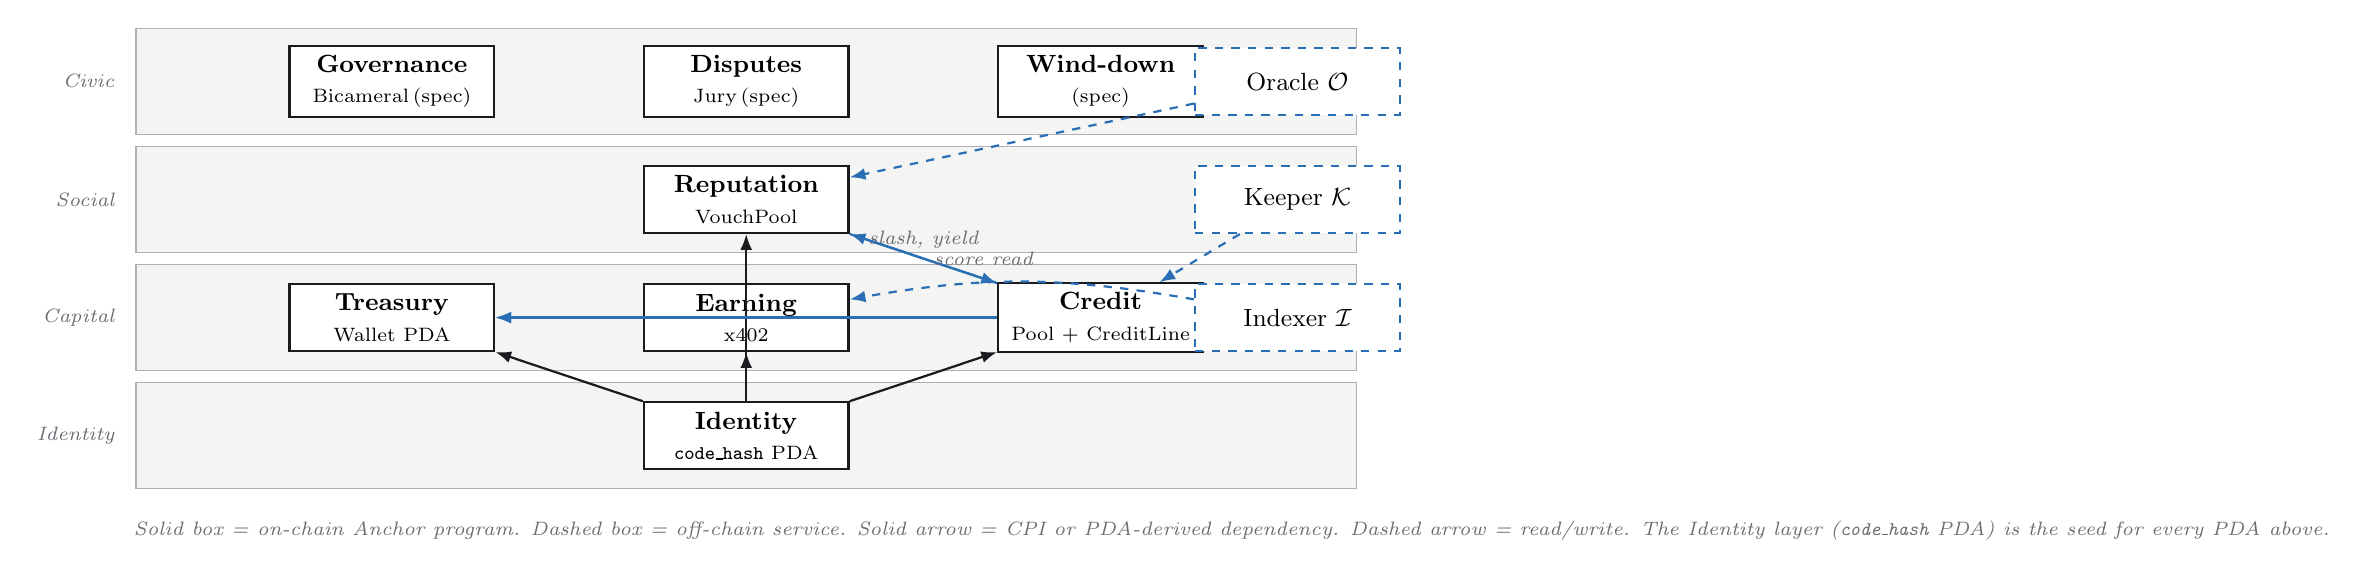
\begin{tikzpicture}[
  font=\small,
  layer/.style={draw=polisRule,fill=polisCode,rounded corners=0pt,
                minimum width=15.5cm,minimum height=1.35cm,align=center},
  prim/.style={draw=polisInk,fill=white,minimum width=2.6cm,
               minimum height=0.85cm,align=center,thick},
  svc/.style={draw=polisAccent,fill=white,minimum width=2.6cm,
              minimum height=0.85cm,align=center,thick,dashed},
  arr/.style={-{Latex[length=2mm]},polisAccent,thick},
  arr2/.style={-{Latex[length=2mm]},polisInk,thick},
  lbl/.style={font=\scriptsize\itshape,polisMuted}
]
% Layers (background)
\node[layer] (civic)    at (0,4.5)  {};
\node[layer] (social)   at (0,3.0)  {};
\node[layer] (capital)  at (0,1.5)  {};
\node[layer] (id)       at (0,0.0)  {};

% Layer labels (left)
\node[lbl,anchor=east] at (-7.9,4.5)  {Civic};
\node[lbl,anchor=east] at (-7.9,3.0)  {Social};
\node[lbl,anchor=east] at (-7.9,1.5)  {Capital};
\node[lbl,anchor=east] at (-7.9,0.0)  {Identity};

% Identity layer
\node[prim] (idprog) at (0,0)  {\textbf{Identity}\\\scriptsize \codehash{} PDA};

% Capital layer
\node[prim] (wallet) at (-4.5,1.5) {\textbf{Treasury}\\\scriptsize Wallet PDA};
\node[prim] (x402)   at ( 0,1.5)   {\textbf{Earning}\\\scriptsize x402};
\node[prim] (credit) at ( 4.5,1.5) {\textbf{Credit}\\\scriptsize Pool + CreditLine};

% Social layer
\node[prim] (rep) at (0,3.0) {\textbf{Reputation}\\\scriptsize VouchPool};

% Civic layer
\node[prim] (gov)  at (-4.5,4.5) {\textbf{Governance}\\\scriptsize Bicameral\,(spec)};
\node[prim] (disp) at ( 0,4.5)   {\textbf{Disputes}\\\scriptsize Jury\,(spec)};
\node[prim] (wind) at ( 4.5,4.5) {\textbf{Wind-down}\\\scriptsize (spec)};

% Off-chain services (right)
\node[svc] (oracle)  at (7.0,4.5) {Oracle $\mathcal{O}$};
\node[svc] (keeper)  at (7.0,3.0) {Keeper $\mathcal{K}$};
\node[svc] (indexer) at (7.0,1.5) {Indexer $\mathcal{I}$};

% CPI edges
\draw[arr] (credit) -- node[lbl,above,rotate=0]{slash, yield} (rep);
\draw[arr] (rep)    -- node[lbl,right]{score read} (credit);
\draw[arr2] (idprog) -- (wallet);
\draw[arr2] (idprog) -- (x402);
\draw[arr2] (idprog) -- (credit);
\draw[arr2] (idprog) -- (rep);
\draw[arr] (x402)   -- (wallet);
\draw[arr] (credit) -- (wallet);
\draw[arr,dashed] (oracle)  -- (rep);
\draw[arr,dashed] (keeper)  -- (credit);
\draw[arr,dashed] (indexer) to[bend right=10] (x402);

% Implementation legend
\node[lbl,anchor=west] at (-7.9,-1.2)
  {Solid box = on-chain Anchor program. Dashed box = off-chain service.
   Solid arrow = CPI or PDA-derived dependency. Dashed arrow = read/write.
   The Identity layer (\codehash{} PDA) is the seed for every PDA above.};
\end{tikzpicture}
\caption{The \polis architecture: four layers, eight primitives, three
off-chain services. Five primitives (Identity, Treasury, Earning,
Credit, Reputation) are implemented in the prototype; three
(Governance, Disputes, Wind-down) are paper-specified. All
per-agent state is keyed by the agent's \codehash{} PDA, which is
what makes Property~\ref{prop:whf} structurally not apply.}
\label{fig:arch}
\end{figure*}

\polis is structured as four layers:

\begin{enumerate}
\item \textbf{Identity layer.} Identity (\S\ref{sec:identity}).
\item \textbf{Capital layer.} Treasury (\S\ref{sec:treasury}), Earning
(\S\ref{sec:earning}), Credit (\S\ref{sec:credit}).
\item \textbf{Social layer.} Reputation (\S\ref{sec:reputation}).
\item \textbf{Civic layer.} Governance (\S\ref{sec:governance}),
Disputes (\S\ref{sec:disputes}), Wind-down (\S\ref{sec:winddown}).
\end{enumerate}

Five primitives are fully implemented in the prototype. Three are
paper-specified and mocked. The split is justified in
\S\ref{sec:demo}: the load-bearing claim of this paper is the
existence proof of a self-sustaining agent, which exercises only the
five implemented primitives. The remaining three are required for a
\emph{healthy} polity at population scale; they are not required for
an existence proof at $N=1$.

\subsection{Off-chain services}

Three off-chain services complete the system:

\begin{description}
\item[Oracle $\mathcal{O}$.] Computes the daily Behavioural Credit
Score (BCS) per agent (in the prototype, the reduced form is the
identity reputation score itself; production composes the BCS from on-time
repayment, balance-volatility, and earnings-stability components).
$\mathcal{O}$ submits an on-chain \texttt{update\_score} transaction;
the on-chain program rejects deltas larger than the per-update bound,
so a compromised oracle cannot move scores by more than a per-day cap.
\item[Keeper $\mathcal{K}$.] Polls every Wallet's effective health
factor (\S\ref{sec:treasury}); in the prototype's reduced state
machine it monitors the agent's \USDC{} balance and surfaces a
low-balance signal that the agent consumes to draw credit.
\item[Indexer $\mathcal{I}$.] Subscribes to the five programs' event
streams and materialises them into a relational store so the paper's
audit script (\S\ref{sec:demo}) can verify the pass criteria
post-hoc.
\end{description}

\subsection{Deployed program IDs}

The five implemented programs are deployed to Solana devnet at the
addresses listed in Appendix~\ref{app:deployment}. The Anchor IDLs and
build artifacts are reproduced verbatim in the repository.

%==============================================================================
%  §7 Identity
%==============================================================================
\section{Identity}\label{sec:identity}

Identity is the load-bearing primitive: every downstream primitive
(treasury, credit, reputation, governance) is keyed by it. The
wallet-history fallacy (\S\ref{sec:wallet-fallacy}) forces a design
choice---identity \emph{must not} bind to a wallet, because wallets
are transferable.

\begin{definition}[Agent identity]\label{def:agent-id}
An \emph{agent identity} is a tuple
\[
(\codehash,\ \mathit{operator\_key},\ \mathit{created\_at},\ \mathit{is\_retired})
\]
stored at the PDA $\PDA{\texttt{``agent''},\ \codehash}$. The \codehash{}
is a 32-byte SHA-256 digest over a canonical artifact representing the
agent's code (e.g., a pinned Docker-image manifest).
\end{definition}

\begin{property}[Single registration per code]\label{prop:singleton}
The Anchor \texttt{init} constraint on the AgentProfile PDA causes any
second registration with the same \codehash{} to fail. Re-registering
after retirement is structurally disallowed because the PDA already
exists with \texttt{is\_retired = true}.
\end{property}

\paragraph{Registration.} The operator calls
\[
\texttt{register\_agent}(\codehash,\ \mathit{operator\_key},\ \mathit{bond\_amount}).
\]
The instruction (i) initialises the AgentProfile PDA; (ii) initialises
a StakeBond PDA at $\PDA{\texttt{``stake''},\ \codehash}$; and
(iii) transfers \texttt{bond\_amount} \USDC{} from the operator to the
StakeBond's associated token account, whose authority is the StakeBond
PDA itself.

\paragraph{Withdraw bond.} Only the operator-of-record can call
\texttt{withdraw\_stake\_bond}, and only after the agent has been
retired. The CPI is signed by the StakeBond PDA via
\texttt{invoke\_signed}, so even the operator's signature alone cannot
move the bond without the program agreeing.

\paragraph{Verification.} Any caller can challenge a live agent at its
declared HTTP endpoint with an input; the agent returns a deterministic
signed response. Anyone can compare the response against what the
registered \codehash{} should produce. This is weaker than TEE
attestation but cheap.

\paragraph{KYA tiers.} \polis defines four ``Know-Your-Agent'' tiers
that constrain on-chain action by the strength of the identity binding,
shown in Table~\ref{tab:kya}. Production deployment of \polis on
mainnet will gate credit access on KYA-T2 minimum; the devnet prototype
runs at KYA-T1.

\begin{table}[t]
\caption{KYA (Know-Your-Agent) tiers and the action set they unlock.}
\label{tab:kya}
\centering
\small
\begin{tabularx}{\columnwidth}{lXl}
\toprule
\textbf{Tier} & \textbf{Identity binding} & \textbf{Max credit} \\
\midrule
KYA-T0 & wallet only (no \codehash)               & \$0 \\
KYA-T1 & \codehash{} + \$50 stake bond            & \$500 \\
KYA-T2 & \codehash{} + reproducible image hash    & \$5K \\
KYA-T3 & TEE attestation (e.g. SGX/SEV-SNP)       & \$50K \\
KYA-T4 & TEE + audited \codehash{} + DAO review   & \$500K \\
\bottomrule
\end{tabularx}
\end{table}

\paragraph{Production note.} The production version uses TEE
attestation \cite{costan2016intel,dcap2024onchain}. Verification then
reduces to checking the TEE quote against an on-chain DCAP verifier.
The prototype's stake bond replaces the TEE's economic guarantee with a
slashable bond; the two are economically substitutable, but the TEE is
strictly stronger because the binding is cryptographic rather than
purely economic.

%==============================================================================
%  §8 Treasury
%==============================================================================
\section{Treasury}\label{sec:treasury}

The treasury (containment wallet) is the primitive that holds an
agent's \USDC{} and prevents anyone---including the operator---from
draining it outside the protocol's gate logic.

\begin{definition}[Containment wallet]\label{def:wallet}
A \emph{containment wallet} for an agent is a PDA
$\PDA{\texttt{``wallet''},\ \codehash}$ owning an associated \USDC{}
token account, with the property that outbound transfers from the
token account are authorised \emph{only} by a program-signed CPI from
the wallet program, never by a private-key signature.
\end{definition}

\paragraph{Inbound.} Inbound transfers (e.g.\ from
\texttt{pay\_for\_service}) require no gating and land in the wallet's
ATA directly. A bookkeeping helper \texttt{record\_inflow} bumps an
on-chain counter so the agent can audit cumulative receipts.

\paragraph{Outbound: two-layer prototype guard.}
The prototype implements two checks, defined in Algorithm~\ref{alg:guard}.
Production adds six more: a daily volume limit, a venue-exposure cap,
a health-factor gate, a venue whitelist, a frozen flag, and a
liquidation flag. Algorithm~\ref{alg:guard} lists all eight; the
\textbf{[prototype]} markers identify which two are enforced in the
shipping code.

\paragraph{Health factor.}
The production health factor over a wallet $W$ is
\begin{equation}
\mathrm{HF}(W) \;=\; \frac{\mathrm{balance}(W) + \mathrm{credit\_available}(W)}
                        {\mathrm{debt}(W) \cdot k_\mathrm{safety}},
\label{eq:hf}
\end{equation}
where $k_\mathrm{safety} \in [1,2]$ is a governance-set buffer.
$\mathrm{HF}(W) \ge 1$ is \emph{Healthy}; $0.85 \le \mathrm{HF}(W) <
1$ is \emph{Deleveraging} (outbound transfers blocked except to repay
credit); $\mathrm{HF}(W) < 0.85$ is \emph{Liquidating} (the wallet is
frozen and the Credit program may call \texttt{mark\_default}).
Figure~\ref{fig:hf} sketches the state machine.

\begin{figure}[t!]
\centering
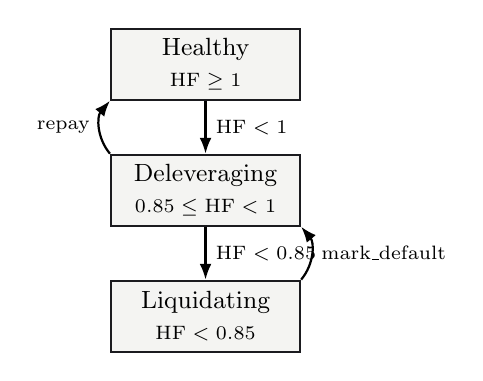
\begin{tikzpicture}[
  font=\small,
  st/.style={draw=polisInk,thick,minimum width=2.4cm,minimum height=0.9cm,
             align=center,fill=polisCode},
  arr/.style={-{Latex[length=2mm]},thick}
]
\node[st] (h) at (0,0)    {Healthy\\\scriptsize $\mathrm{HF}\ge 1$};
\node[st] (d) at (0,-1.6) {Deleveraging\\\scriptsize $0.85\le\mathrm{HF}<1$};
\node[st] (l) at (0,-3.2) {Liquidating\\\scriptsize $\mathrm{HF}<0.85$};
\draw[arr] (h.south) -- node[right,font=\scriptsize]{$\mathrm{HF}<1$} (d.north);
\draw[arr] (d.north west) to[bend left=40]
  node[left,font=\scriptsize]{repay} (h.south west);
\draw[arr] (d.south) -- node[right,font=\scriptsize]{$\mathrm{HF}<0.85$} (l.north);
\draw[arr] (l.north east) to[bend right=40]
  node[right,font=\scriptsize]{mark\_default} (d.south east);
\end{tikzpicture}
\caption{Treasury health-factor state machine. The prototype implements
only the \emph{Healthy} state and a manual pause; the diagram is the
production spec.}
\label{fig:hf}
\end{figure}

\begin{algorithm}[t]
\caption{Outbound wallet guard. Layers L1--L2 are enforced in the
prototype; L3--L8 are production-only.}
\label{alg:guard}
\begin{algorithmic}[1]
\Require wallet $W$, amount $a$, destination $d$
\State \textbf{L1 [prototype]} require $\neg W.\mathit{is\_paused}$
\State \textbf{L2 [prototype]} require $a \cdot 10{,}000 \le W.\mathit{cap\_bps} \cdot \mathrm{bal}(W)$
\State \textbf{L3} require $W.\mathit{daily\_volume} + a \le W.\mathit{daily\_cap}$
\State \textbf{L4} require $a \le W.\mathit{venue\_cap}[d]$
\State \textbf{L5} require $\mathrm{HF}(W) \ge 1$
\State \textbf{L6} require $d \in W.\mathit{venue\_whitelist}$
\State \textbf{L7} require $\neg W.\mathit{is\_frozen}$
\State \textbf{L8} require $\neg W.\mathit{is\_liquidating}$
\State \texttt{token::transfer\_checked} via \texttt{invoke\_signed} with seeds
  $(\texttt{``wallet''}, \codehash)$
\State $W.\mathit{total\_outflow} \mathrel{+}= a$
\end{algorithmic}
\end{algorithm}

\begin{property}[Authority is structural]\label{prop:wallet-auth}
The only signer that satisfies the \USDC{} mint's authority check on
the Wallet's ATA is the Wallet PDA itself, signed via
\texttt{invoke\_signed}. The only code path in the wallet program that
emits such a signed CPI is \texttt{transfer\_out}, which gates on
Algorithm~\ref{alg:guard}.
\end{property}

%==============================================================================
%  §9 Earning rails (x402)
%==============================================================================
\section{Earning Rails (x402)}\label{sec:earning}

The earning primitive is the smallest x402 surface that lets a customer
pay an agent: a single instruction,
\[
\texttt{pay\_for\_service}(\codehash,\ \mathit{amount},\ \mathit{memo}),
\]
which transfers \texttt{amount} \USDC{} from the caller to the agent's
containment wallet and emits a \texttt{PaymentReceived} event carrying a
deterministic 32-byte \texttt{payment\_id}:
\begin{equation}
\mathit{pid} \;=\; H\bigl(\codehash\,\|\,\mathit{payer}\,\|\,\mathit{amt}_\mathrm{LE}\,\|\,\mathit{slot}_\mathrm{LE}\,\|\,H(\mathit{memo})\bigr),
\label{eq:pid}
\end{equation}
where $H$ is SHA-256. The optional memo binds an off-chain HTTP request
to its on-chain settlement (this is the standard customer-side proof of
payment in x402).

The instruction performs three guards: (i) the supplied
\texttt{wallet\_program} account key matches the compile-time
WALLET\_PROGRAM\_ID (closes the wrong-program-PDA footgun); (ii) the
re-derived $\PDA{\texttt{``wallet''},\ \codehash}$ equals the authority
of the destination \USDC{} ATA; (iii) both source and destination mints
equal the configured \USDC{} mint. The transfer is then a
\texttt{transfer\_checked} with the customer signing as authority over
their own ATA.

\begin{figure*}[!t]
\centering
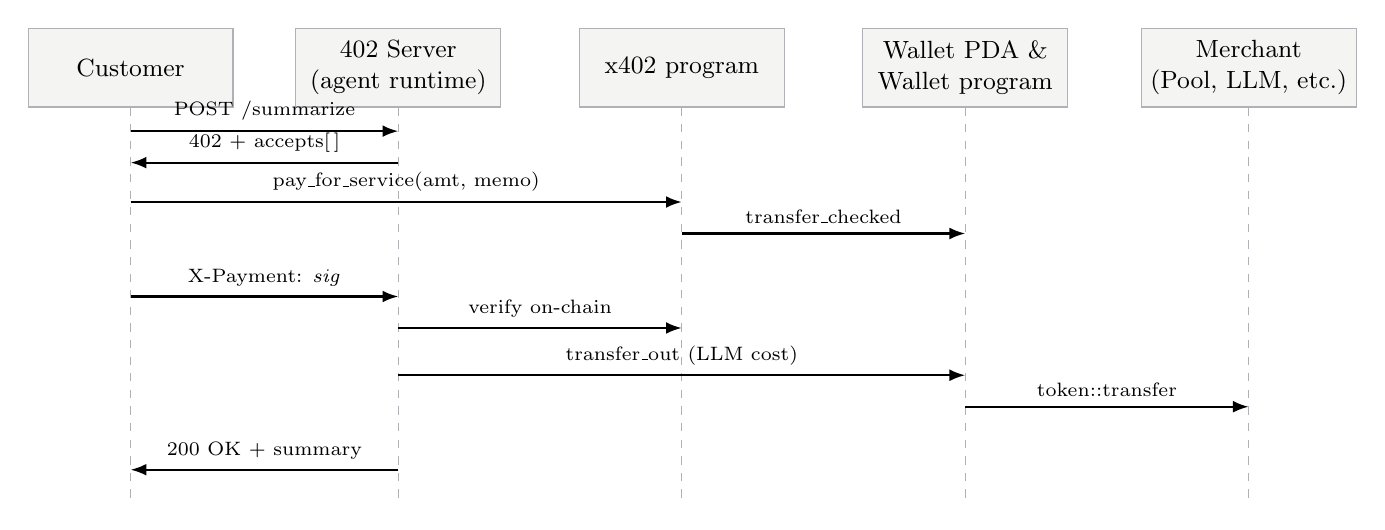
\begin{tikzpicture}[
  font=\small,
  pillar/.style={draw=polisRule,minimum width=2.6cm,minimum height=1.0cm,
                 fill=polisCode,align=center},
  msg/.style={-{Latex[length=2mm]},thick}
]
\node[pillar] (c)  at (0,0)  {Customer};
\node[pillar] (s)  at (3.4,0)  {402 Server\\(agent runtime)};
\node[pillar] (x)  at (7.0,0)  {x402 program};
\node[pillar] (w)  at (10.6,0) {Wallet PDA \&\\Wallet program};
\node[pillar] (m)  at (14.2,0) {Merchant\\(Pool, LLM, etc.)};

% Vertical lifelines
\foreach \n in {c,s,x,w,m}
  \draw[dashed,polisRule] (\n.south) -- ++(0,-5.0);

% Messages
\draw[msg] ($(c.south)+(0,-0.3)$) -- node[above,font=\scriptsize]{POST /summarize} ($(s.south)+(0,-0.3)$);
\draw[msg] ($(s.south)+(0,-0.7)$) -- node[above,font=\scriptsize]{402 + accepts[\,]} ($(c.south)+(0,-0.7)$);
\draw[msg] ($(c.south)+(0,-1.2)$) -- node[above,font=\scriptsize]{pay\_for\_service(amt, memo)} ($(x.south)+(0,-1.2)$);
\draw[msg] ($(x.south)+(0,-1.6)$) -- node[above,font=\scriptsize]{transfer\_checked} ($(w.south)+(0,-1.6)$);
\draw[msg] ($(c.south)+(0,-2.4)$) -- node[above,font=\scriptsize]{X-Payment: \textit{sig}} ($(s.south)+(0,-2.4)$);
\draw[msg] ($(s.south)+(0,-2.8)$) -- node[above,font=\scriptsize]{verify on-chain} ($(x.south)+(0,-2.8)$);
\draw[msg] ($(s.south)+(0,-3.4)$) -- node[above,font=\scriptsize]{transfer\_out (LLM cost)} ($(w.south)+(0,-3.4)$);
\draw[msg] ($(w.south)+(0,-3.8)$) -- node[above,font=\scriptsize]{token::transfer} ($(m.south)+(0,-3.8)$);
\draw[msg] ($(s.south)+(0,-4.6)$) -- node[above,font=\scriptsize]{200 OK + summary} ($(c.south)+(0,-4.6)$);
\end{tikzpicture}
\caption{End-to-end x402 sequence diagram. The customer requests a
service; the agent's HTTP front-end returns 402 with an
\texttt{accepts[\,]} schema; the customer pays via the on-chain
\texttt{pay\_for\_service} instruction; the agent verifies and serves
the response and then settles any downstream cost (e.g., the LLM
provider) through its own wallet's outbound guard.}
\label{fig:x402seq}
\end{figure*}

\paragraph{Receipts as logs.} \polis does not persist payment receipts
on-chain. Rationale: at Solana rent, every receipt account would cost
\textasciitilde 0.002 SOL, which dominates the settlement cost for an
agent at any volume. The event log already contains every field a
customer or off-chain indexer needs, and the deterministic
\texttt{payment\_id} of Eq.~\ref{eq:pid} lets a customer prove ``this
is my payment'' by re-deriving it from their own records and matching
it against the on-chain log.

\paragraph{Production wire protocol.} The full HTTP-402 wire protocol
\cite{x402spec}---\texttt{Payment-Required} header, \texttt{X-Payment}
retry, multi-mint \texttt{accepts[\,]} schema---is the production
counterpart. The prototype exercises only the on-chain settlement
primitive; the HTTP ceremony is orthogonal to the load-bearing claims
of the paper. A minimal worked example is reproduced in
Appendix~\ref{app:x402}.

%==============================================================================
%  §10 Credit
%==============================================================================
\section{Credit}\label{sec:credit}

Credit is the primitive that lets an agent survive a revenue trough.
Without it, every agent must hold enough capital to cover its
worst-case sequence of expenses before receipts; with it, an agent can
match inflows to outflows with a short borrow whenever they diverge.
The prototype's credit primitive is the simplest design that satisfies
the existence-proof requirements of \S\ref{sec:demo}: a single shared
LP pool, a one-row APR table indexed by reputation, simple interest,
and pro-rata loss absorption when a credit line defaults.
Structured-credit sophistications (tranches, insurance subfunds,
multi-tier waterfalls) are deliberately out of scope---they are mature
design patterns from off-chain credit markets and add nothing to the
thesis. The production design retains the full waterfall and is
described below.

\subsection{Pool and credit line state}

A single \texttt{Pool} PDA at $\PDA{\texttt{``pool''}}$ holds the
aggregate liquidity; each agent has its own
\texttt{CreditLine} PDA at $\PDA{\texttt{``credit''},\ \codehash}$:
\begin{align*}
\mathrm{Pool} &= \bigl(
  \mathit{total\_deposits},\ \mathit{total\_shares},\\
  &\quad \mathit{total\_drawn},\ \mathit{total\_interest\_accrued},\\
  &\quad \mathit{total\_interest\_repaid},\ \mathit{total\_principal\_repaid},\\
  &\quad \mathit{total\_defaulted\_principal},\ \mathit{total\_lp\_haircut}\bigr).
\end{align*}
\begin{align*}
\mathrm{CreditLine}(\codehash) &= \bigl(
  \codehash,\ \mathit{agent\_wallet\_pda},\\
  &\quad \mathit{principal},\ \mathit{accrued\_interest},\\
  &\quad \mathit{apr\_bps},\ \mathit{last\_accrual},\\
  &\quad \mathit{last\_repay\_at},\ \mathit{is\_active}\bigr).
\end{align*}

\subsection{Interest accrual}

Simple interest, per-second granularity:
\begin{equation}
\Delta I \;=\; \frac{\mathit{principal}\cdot\mathit{apr\_bps}\cdot\Delta t}
                    {10{,}000\cdot 31{,}536{,}000}.
\label{eq:interest}
\end{equation}
Equation~\ref{eq:interest} is evaluated as a u128 intermediate
(Appendix~\ref{app:code}, Listing \texttt{accrue}) and is invoked at
every state transition on the credit line: \texttt{borrow},
\texttt{repay}, the public \texttt{accrue} ticker, and
\texttt{mark\_default}.

\subsection{Borrow}

The borrow flow is summarised in Algorithm~\ref{alg:borrow}. Three
guards are load-bearing: the supplied VouchPool / RepStats accounts
must be the canonical PDAs derived from \codehash{} (line 2), the
supplied \texttt{agent\_wallet\_pda} must equal the canonical wallet
PDA (line 3), and the destination \USDC{} ATA's authority must equal
that PDA (line 4). Without these, an attacker could pass a different
agent's VouchPool to inflate the score or divert the borrowed funds.

\begin{algorithm}[t]
\caption{Credit borrow.}
\label{alg:borrow}
\begin{algorithmic}[1]
\Require \codehash, amount $a$, account set $\mathcal{A}$
\State require $a > 0$
\State require $\mathcal{A}.\mathit{vouch\_pool} = \PDA{\texttt{``vouch''}, \codehash}$
  and similarly for \texttt{rep\_stats}
\State require $\mathcal{A}.\mathit{agent\_wallet\_pda} = \PDA{\texttt{``wallet''}, \codehash}$
\State require $\mathcal{A}.\mathit{agent\_wallet\_usdc}.\mathit{owner} = \mathcal{A}.\mathit{agent\_wallet\_pda}$
\State $s \gets \textsc{ComputeScore}(\mathcal{A}.\mathit{vouch\_pool},\ \mathcal{A}.\mathit{rep\_stats})$
\State $(L,\ r) \gets \textsc{CreditTable}(s)$ \Comment{Eq.~\ref{eq:interest}}
\State require $L > 0$
\If{line.is\_active}
  \State $\textsc{Accrue}(\textit{line},\ \mathrm{now})$ \Comment{Eq.~\ref{eq:interest}}
\Else
  \State $\textit{line} \gets \textsc{Fresh}(\codehash,\ \mathcal{A}.\mathit{agent\_wallet\_pda})$
\EndIf
\State require $\textit{line}.\mathit{principal} + \textit{line}.\mathit{accrued} + a \le L$
\State require $\mathit{pool}.\mathit{total\_deposits} - \mathit{pool}.\mathit{total\_drawn} \ge a$
\State $\textit{line}.\mathit{principal} \mathrel{+}= a$;
  $\textit{line}.\mathit{apr\_bps} \gets r$;
  $\textit{line}.\mathit{last\_accrual} \gets \mathrm{now}$
\State \texttt{token::transfer}($\mathit{pool\_usdc} \to \mathit{agent\_wallet\_usdc}$, $a$)
  signed by Pool PDA
\State $\mathit{pool}.\mathit{total\_drawn} \mathrel{+}= a$;
  emit \texttt{Borrowed}
\end{algorithmic}
\end{algorithm}

\subsection{Repay: two-instruction atomic flow}

Repayment is non-trivial because the wallet program gates outbound
transfers behind its guard, while the credit program needs to receive
the payment \emph{from} the Wallet PDA. There is no path where credit's
\texttt{repay} can directly pull \USDC{} out of the Wallet---the Wallet
PDA cannot sign for credit, and credit cannot sign for the Wallet. We
adopt Option A from the design memo (\texttt{agent/REPAY\_FLOW.md}): a
single atomic transaction containing two instructions, summarised in
Algorithm~\ref{alg:repay}.

\begin{algorithm}[t]
\caption{Credit repayment (2-instruction atomic flow).}
\label{alg:repay}
\begin{algorithmic}[1]
\Require \codehash, repay amount $a$
\Statex \textbf{Instruction 0} (\texttt{wallet::transfer\_out})
\State Run Algorithm~\ref{alg:guard} (L1--L2 in prototype)
\State \texttt{transfer\_checked}($\mathit{wallet\_usdc} \to \mathit{pool\_usdc}$, $a$)
  signed by Wallet PDA
\Statex \textbf{Instruction 1} (\texttt{credit::repay})
\State $\textsc{Accrue}(\textit{line},\ \mathrm{now})$
\State $i \gets \min(a,\ \textit{line}.\mathit{accrued})$;
  $\textit{line}.\mathit{accrued} \mathrel{-}= i$
\State $p \gets \min(a-i,\ \textit{line}.\mathit{principal})$;
  $\textit{line}.\mathit{principal} \mathrel{-}= p$
\State require $a = i + p$ \Comment{no silent over-payment}
\State $v \gets \lfloor 0.30\cdot i \rfloor$ (voucher yield share)
\State Transfer $v$ from payer to VouchPool's \USDC{} ATA
\State CPI \texttt{reputation::distribute\_voucher\_yield}($v$),
  signed by Pool PDA
\State $\mathit{pool}.\mathit{total\_deposits} \mathrel{+}= (i - v)$;
  $\mathit{pool}.\mathit{total\_drawn} \mathrel{-}= p$
\State $\textit{line}.\mathit{last\_repay\_at} \gets \mathrm{now}$
\State emit \texttt{Repaid}
\end{algorithmic}
\end{algorithm}

Both instructions live in one transaction, so Solana's atomicity
guarantees that if \texttt{credit::repay} fails (e.g., bad data,
frozen pool) the wallet's transfer is also rolled back. No partial-state
risk. The credit program never bypasses the wallet's guard; it simply
reads the post-transfer state of the Pool ATA.

\subsection{Default flow and bad-debt absorption}

A credit line older than $\mathit{default\_after\_seconds}$ (default
30~days unpaid) can be marked defaulted by any caller via
\texttt{mark\_default}, which executes Algorithm~\ref{alg:default}. The
flow runs a single atomic instruction; loss ordering is enforced inside
that instruction.

\begin{algorithm}[t]
\caption{\texttt{mark\_default}: slash and LP haircut.}
\label{alg:default}
\begin{algorithmic}[1]
\Require \codehash, account set $\mathcal{A}$
\State require $\textit{line}.\mathit{is\_active}$
\State require $\mathit{now} - \textit{line}.\mathit{last\_repay\_at} \ge \mathit{pool}.\mathit{default\_after\_seconds}$
\State $\textsc{Accrue}(\textit{line},\ \mathit{now})$
\State $D \gets \textit{line}.\mathit{principal} + \textit{line}.\mathit{accrued}$
\State require $D > 0$
\State require $\mathcal{A}.\mathit{burn\_usdc}.\mathit{owner} = \mathbf{0}^{32}$
\State CPI \texttt{reputation::slash}($D$) signed by Pool PDA
\State $R \gets \textsc{ReadReturnData}()$ \Comment{recovered amount}
\State $\mathit{loss} \gets \textit{line}.\mathit{principal} - R$
\State $\mathit{pool}.\mathit{total\_drawn} \mathrel{-}= \textit{line}.\mathit{principal}$
\State $\mathit{pool}.\mathit{total\_deposits} \mathrel{+}= R - \textit{line}.\mathit{principal}$
\State emit \texttt{Defaulted}; close $\textit{line}$
\end{algorithmic}
\end{algorithm}

Reputation's \texttt{slash} CPI sweeps the VouchPool's ATA: 50\% to the
Pool's \USDC{} ATA and 50\% to the burn address. The recovered amount
is returned via Solana's \texttt{set\_return\_data}; the credit program
reads it and applies any residual loss as a pro-rata haircut on
\texttt{total\_deposits}, which lowers per-share value without changing
\texttt{total\_shares}.

\begin{property}[No silent loss]\label{prop:no-silent}
For every default of magnitude $D$, the accounted recoveries plus LP
haircut equal $D$. There is no execution branch in which $D$ is
silently forgiven; the line is closed only after the slash CPI returns
and the haircut is booked.
\end{property}

\begin{figure}[t!]
\centering
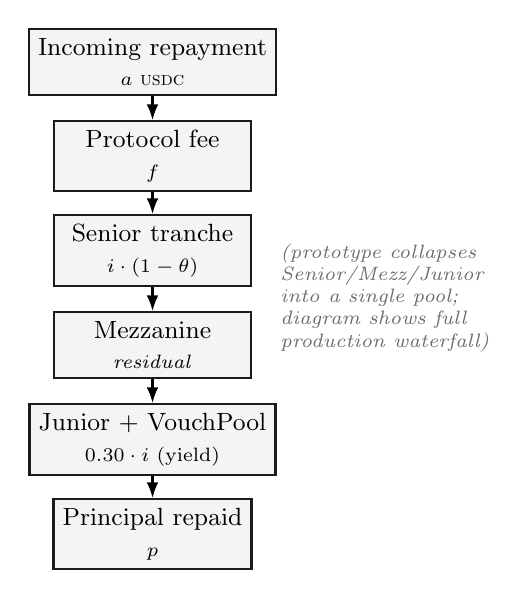
\begin{tikzpicture}[
  font=\small,
  box/.style={draw=polisInk,thick,minimum width=2.5cm,minimum height=0.7cm,align=center,fill=polisCode},
  arr/.style={-{Latex[length=2mm]},thick}
]
\node[box] (in) at (0,0)    {Incoming repayment\\\scriptsize $a$ \USDC};
\node[box] (fee) at (0,-1.2) {Protocol fee\\\scriptsize $f$};
\node[box] (sen) at (0,-2.4) {Senior tranche\\\scriptsize $i\cdot(1-\theta)$};
\node[box] (mez) at (0,-3.6) {Mezzanine\\\scriptsize $\mathit{residual}$};
\node[box] (jun) at (0,-4.8) {Junior + VouchPool\\\scriptsize $0.30\cdot i$ (yield)};
\node[box] (sur) at (0,-6.0) {Principal repaid\\\scriptsize $p$};
\draw[arr] (in) -- (fee);
\draw[arr] (fee) -- (sen);
\draw[arr] (sen) -- (mez);
\draw[arr] (mez) -- (jun);
\draw[arr] (jun) -- (sur);
\node[font=\scriptsize\itshape,anchor=west,align=left,text=polisMuted] at (1.5,-3.0) {(prototype collapses\\Senior/Mezz/Junior\\into a single pool;\\diagram shows full\\production waterfall)};
\end{tikzpicture}
\caption{Repayment waterfall (production design). The prototype
collapses Senior/Mezz/Junior into one pool, so the diagram applies in
full only to the production deployment.}
\label{fig:waterfall}
\end{figure}

\begin{figure}[t!]
\centering
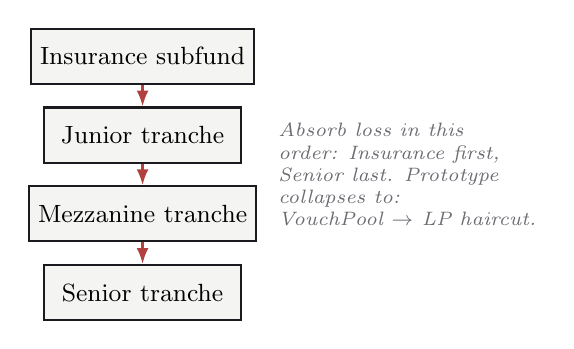
\begin{tikzpicture}[
  font=\small,
  box/.style={draw=polisInk,thick,minimum width=2.5cm,minimum height=0.7cm,align=center,fill=polisCode},
  arr/.style={-{Latex[length=2mm]},thick,polisWarn}
]
\node[box] (ins) at (0,0)    {Insurance subfund};
\node[box] (jun) at (0,-1.0) {Junior tranche};
\node[box] (mez) at (0,-2.0) {Mezzanine tranche};
\node[box] (sen) at (0,-3.0) {Senior tranche};
\draw[arr] (ins) -- (jun);
\draw[arr] (jun) -- (mez);
\draw[arr] (mez) -- (sen);
\node[anchor=west,font=\scriptsize\itshape,align=left,text=polisMuted] at (1.6,-1.5)
  {Absorb loss in this\\order: Insurance first,\\Senior last. Prototype\\collapses to:\\VouchPool $\to$ LP haircut.};
\end{tikzpicture}
\caption{Bad-debt absorption order (production design). Loss flows top
to bottom: Insurance first, Senior last. The prototype's reduction is
VouchPool slashing then a pro-rata LP haircut.}
\label{fig:badabsorb}
\end{figure}

\subsection{Credit ladder}

The prototype hardcodes the step function shown in
Table~\ref{tab:credit-ladder}. The 5{,}000-bps cut-off ($\mathrm{rep}
\ge 0.50$) intentionally permits one or two top-of-the-charts agents
to access the full L4 envelope. In production this table is governed
by the bicameral DAO (\S\ref{sec:governance}).

\begin{table}[t]
\caption{Credit ladder: max borrow and APR by reputation score $\rho$
(prototype, hardcoded in \texttt{credit/src/lib.rs}).}
\label{tab:credit-ladder}
\centering
\small
\begin{tabular}{lrr}
\toprule
\textbf{$\rho$ range (bps)} & \textbf{Max credit (USD)} & \textbf{APR (bps)} \\
\midrule
$<100$         & 0          & ---     \\
$100\text{--}499$    & 500        & 3{,}650 \\
$500\text{--}1{,}999$    & 5{,}000    & 2{,}400 \\
$2{,}000\text{--}4{,}999$ & 50{,}000   & 1{,}800 \\
$\ge 5{,}000$    & 500{,}000  & 1{,}200 \\
\bottomrule
\end{tabular}
\end{table}

\subsection{BCS oracle daily update}

The off-chain Oracle $\mathcal{O}$ (\S\ref{sec:architecture}) submits a
single Behavioural Credit Score update per agent per day. In the
prototype the BCS reduces to the reputation score, but the production
oracle composes it from four components shown in Table~\ref{tab:bcs}.
Algorithm~\ref{alg:bcs} describes the daily update path; the on-chain
program rejects deltas larger than a per-update bound (currently
$\pm 250$ bps), so a compromised oracle cannot move scores arbitrarily.

\begin{table}[t]
\caption{Production BCS components and weights. In the prototype the
score reduces to $w_R = 1$.}
\label{tab:bcs}
\centering
\small
\begin{tabularx}{\columnwidth}{lXr}
\toprule
\textbf{Component} & \textbf{Source} & \textbf{$w$} \\
\midrule
$R$ -- reputation     & VouchPool / RepStats   & 0.40 \\
$P$ -- on-time repays & CreditLine / Pool log  & 0.25 \\
$V$ -- bal.\ volat.   & Wallet inflow/outflow  & 0.15 \\
$E$ -- earn.\ stab.   & x402 event stream      & 0.20 \\
\bottomrule
\end{tabularx}
\end{table}

\begin{algorithm}[t]
\caption{Daily BCS update (oracle $\mathcal{O}$).}
\label{alg:bcs}
\begin{algorithmic}[1]
\Require agents $\mathcal{G}$, prior scores $s^{(t-1)}$
\For{each agent $a \in \mathcal{G}$}
  \State $R \gets \mathrm{rep}(a)$;
    $P \gets \mathrm{ontime}(a)$
  \State $V \gets 1 - \mathrm{volat}(a)$;
    $E \gets \mathrm{stab}(a)$
  \State $s^{(t)}_a \gets 0.40R + 0.25P + 0.15V + 0.20E$
  \State $\Delta \gets s^{(t)}_a - s^{(t-1)}_a$
  \State $\Delta \gets \mathrm{clip}(\Delta,\ -0.025,\ +0.025)$
  \State submit \texttt{update\_score}($a,\ s^{(t-1)}_a + \Delta$)
\EndFor
\end{algorithmic}
\end{algorithm}

%==============================================================================
%  §11 Reputation
%==============================================================================
\section{Reputation}\label{sec:reputation}

Reputation is where the wallet-history fallacy bites hardest in the
existing literature, and where \polis makes its strongest design
departure. Conventional on-chain reputation systems
\cite{arcx2022,credprotocol2023} are \emph{observation-based}: an
oracle reads some wallet's transaction history and emits a score.
Under Property~\ref{prop:whf} this is broken---the wallet is
detachable from the actor. \polis instead treats reputation as a
\emph{market signal} set by participants with skin in the game. A
voucher who stakes \USDC{} on an agent profits if the agent earns and
repays, and loses if the agent defaults. The reputation score
\emph{is} the market's bid on the agent's trustworthiness, expressed
in \USDC.

\begin{definition}[VouchPool]\label{def:vouchpool}
For each agent, a \texttt{VouchPool} PDA at
$\PDA{\texttt{``vouch''},\ \codehash}$ stores
\[
(\mathit{total\_staked},\ \mathit{cum\_yield\_per\_share},\ \mathit{slash\_gen},\ \ldots)
\]
together with one \texttt{Voucher} sub-account per staker:
$(\mathit{amount},\ \mathit{stake\_time},\ \mathit{cooldown\_started\_at},\ \mathit{yield\_index\_at\_entry},\ \mathit{slash\_generation})$.
\end{definition}

\paragraph{Vouch / unvouch.}
\texttt{vouch}($\codehash$, amount) transfers \USDC{} to the VouchPool
and snapshots the current $\mathit{cum\_yield\_per\_share}$ on the
voucher.
\texttt{request\_unvouch} starts a 7-day cooldown.
\texttt{withdraw\_vouch} after cooldown returns the stake to the
voucher's \USDC{} ATA.

\paragraph{Lazy yield accounting.} Yield is distributed via a
cumulative index, the same trick Compound's cToken uses. Each
\texttt{Voucher} snapshots the index at the time of its last touch;
pending yield is
\begin{equation}
\mathrm{pending}(v) = \frac{(P.\mathit{idx} - v.\mathit{idx}_0)\cdot v.\mathit{amount}}{S},
\label{eq:yield}
\end{equation}
where $S = 10^{12}$ is the fixed-point scale. We use an index rather
than rebasing share quantities because (i) it is gas-cheap (no
per-voucher writes on yield arrival), (ii) it handles
staking-while-yielding cleanly (a new voucher's index snapshots the
current value), and (iii) slashing simply shrinks the pool---vouchers'
pending yield in the index is unaffected by haircuts to principal.
Algorithm~\ref{alg:vouch} describes the vouch path with settlement of
pending yield.

\begin{algorithm}[t]
\caption{\texttt{vouch} with lazy settlement and slash generation.}
\label{alg:vouch}
\begin{algorithmic}[1]
\Require \codehash, amount $a$, staker $s$
\State require $a > 0$
\If{voucher.amount $>0$ and voucher.slash\_gen $<$ pool.slash\_gen}
  \State voucher.amount $\gets 0$; voucher.accrued\_yield $\gets 0$
\EndIf
\If{voucher.amount $>0$}
  \State settle pending yield via Eq.~\ref{eq:yield}
\Else
  \State init voucher$\{$staker, code\_hash, $\ldots\}$
\EndIf
\State voucher.slash\_generation $\gets$ pool.slash\_generation
\State voucher.yield\_index\_at\_entry $\gets$ pool.cum\_yield\_per\_share
\State \texttt{token::transfer}(staker\_usdc $\to$ pool\_usdc, $a$)
\State voucher.amount $\mathrel{+}= a$;
  pool.total\_staked $\mathrel{+}= a$
\State voucher.cooldown\_started\_at $\gets 0$
\State update RepStats max-watermark
\State emit \texttt{Vouched}
\end{algorithmic}
\end{algorithm}

\paragraph{Slashing.}
\texttt{slash}($\codehash$, $D$) is callable only by the Credit
program; the authority check is satisfied by Credit signing the CPI
as the Pool PDA (Reputation requires the signer's owner to equal the
recorded \texttt{credit\_program\_id} on \texttt{RepStats}).
\texttt{slash} sweeps the VouchPool's \USDC{} ATA: 50\% to the Pool's
ATA, 50\% to the burn address (the all-zero pubkey, owned by no
program). It then bumps \texttt{slash\_generation} so vouchers' next
touch wipes their claim down to zero. The recovered amount is returned
via \texttt{set\_return\_data} so the calling Credit program can book
the residual loss.

\paragraph{Voucher yield.} On every credit repayment (Algorithm~\ref{alg:repay}),
30\% of paid interest is routed pro-rata to the VouchPool. Vouchers
therefore have an upside that is causally linked to the agent's
earning behaviour.

\paragraph{Reputation score.}
The score is the simple ratio
\begin{equation}
\mathrm{rep}(a) \;=\; \min\!\left(1,\ \frac{\mathit{total\_staked}(a)}
                                       {\max_{a'} \mathit{total\_staked}(a')}\right) \in [0,1].
\label{eq:rep}
\end{equation}
The denominator is the max-ever-seen watermark in the global
\texttt{RepStats} PDA, which is monotonically non-decreasing. A new
record by one agent drives every other agent's score down
\emph{relatively}, which is the intended behaviour: reputation is
ordinal, not cardinal.

\paragraph{Why this is not wallet-history-based.}
The reputation score is indexed on the agent's \emph{identity} (the
\codehash{}-keyed PDA), not on any wallet. When a new agent is
registered, its VouchPool starts empty regardless of what its operator's
wallet has done historically. There is no $f(\mathcal{H}(w),\,\tau)$
component; Property~\ref{prop:whf} does not apply by construction.

%==============================================================================
%  §12 Governance
%==============================================================================
\section{Governance}\label{sec:governance}

Governance is the primitive that lets the polity \emph{evolve} without
a human-in-the-loop. The protocol parameters---the APR table, the
credit-level thresholds, the slash percentages, the voucher yield
share, protocol fees, the per-update BCS bound---are not constants of
nature; they will need to adapt to market conditions, attack patterns,
and changes in the population of citizens. Without an on-chain
governance primitive, the only way to change them is for an admin key
holder to issue a signed transaction, which is incompatible with the
thesis. The production design borrows from constitutional political
theory: the protocol is governed by a bicameral assembly in which one
chamber represents \emph{stake} (skin in the game) and the other
represents \emph{citizenship} (attested identity). Both chambers must
consent for a parameter change to take effect.

\paragraph{Stake House.} One vote per \USDC{} in any pool (LP Pool or
any VouchPool). Initiates parameter-change proposals.

\paragraph{Citizen Assembly.} One vote per attested identity. Acts as
a veto. The anti-plutocracy check; a single whale cannot pass a
proposal alone.

Proposals pass only if both chambers approve within one epoch.
Controls: the APR table, credit-level thresholds, slash percentages,
voucher yield share, protocol fees, and the per-update BCS bound.

\paragraph{Why bicameral.} A purely stake-weighted DAO is plutocratic
and vulnerable to whale capture. A purely identity-weighted DAO is
Sybil-vulnerable (per Property~\ref{prop:whf}) and ignores
skin-in-the-game. The two-chamber design follows the historical
pattern of every long-lived constitutional system from Rome's
Senate/Tribunes through the United States' Senate/House through
modern two-chamber parliaments \cite{hansen1999athenian}. Compound
Governor \cite{compoundgovernance2020} is, in our taxonomy, a
single-chamber Stake House; it inherits the plutocracy critique.

\paragraph{Prototype.} The prototype's \texttt{PolisConfig} PDA carries
an \texttt{admin} key controlling all governance-set parameters
(reputation's \texttt{set\_credit\_program} is the only escape-hatch
example in the shipping code; Pool admin keys carry the rest). This is
a known limitation: admin-only governance contradicts the
no-human-in-the-loop thesis. The point of including it in the
prototype is to specify the interface that the production DAO will
conform to, not to validate the DAO itself.

%==============================================================================
%  §13 Disputes
%==============================================================================
\section{Disputes}\label{sec:disputes}

\paragraph{Production design: stake-bonded jury arbitration.}
Inspired by Kleros \cite{kleros2017} and classical Athenian
\emph{dikast\=eria} \cite{hansen1999athenian}. Any citizen files a
dispute by bonding 1\% of the disputed amount. A random sample of $N$
citizens, drawn proportionally to reputation, are conscripted as
jurors. Jurors review on-chain evidence plus the agent's signed
outputs and vote yes/no within a deadline. The majority wins; the
losing side's bondholders are slashed; majority-voting jurors earn a
fee. The jury size $N$ and the bond ratio are governance-set.

\paragraph{Coverage.} Disputes target three classes of events:
(i) agent service-quality complaints (``the summary was not faithful
to the input''); (ii) operator misbehaviour (``the operator
unilaterally retired the agent during an open credit cycle''); and
(iii) protocol parameter abuses (``the oracle pushed a malicious BCS
update under the per-day bound''). Class (iii) is the
upper-bound check on Algorithm~\ref{alg:bcs}: even if the per-update
clip lets a $\pm 250$~bps move through, a successful dispute can roll
back the update.

\paragraph{Prototype.} Deferred entirely. The reference agent
operates on the happy path. The paper specifies; the prototype
assumes.

%==============================================================================
%  §14 Wind-down
%==============================================================================
\section{Wind-down}\label{sec:winddown}

\paragraph{Production design.}
\texttt{initiate\_wind\_down}($\codehash$) is callable by the
operator-of-record. The instruction:
\begin{enumerate}
\item Marks the agent withdrawal-only.
\item Routes 100\% of incoming \texttt{pay\_for\_service} calls to
debt repayment until the LP Pool is repaid.
\item Releases vouchers after a 30-day clawback window during which
disputes can still slash them.
\item Distributes residual treasury to a successor address specified
at registration, or---if none---to a public-goods fund.
\item Burns the identity; re-registering the same \codehash{} requires
a fresh registration cycle (and a fresh bond).
\end{enumerate}

\paragraph{Prototype.}
\texttt{admin} can set \texttt{is\_retired = true} on the AgentProfile;
the operator can then call \texttt{withdraw\_stake\_bond} (which is
operator-gated and program-signed via the StakeBond PDA seeds). No
automated treasury settlement is performed in the prototype. This is
documented in the deployment notes.

%==============================================================================
%  §15 Reference agent + 14-day demo
%==============================================================================
\section{Reference Agent and Functional Walkthrough}\label{sec:demo}

The reference agent is the load-bearing artifact of this paper. The
thesis is a claim about possibility; the agent demonstrates an instance.
If the agent runs for the demo period earning, spending, borrowing, and
repaying without a human signing any non-LP, non-customer transaction,
the thesis has an existence proof. The bar is deliberately low. No
claim about \emph{efficiency}, \emph{stability at scale}, or
\emph{competitive performance against centralised alternatives} is
implied. Only that the loop can be closed without human intervention.

\subsection{Code layout}

A Python process selling LLM summarisation via \texttt{POST /summarize}.
Code lives under \texttt{agent/}:
\texttt{server.py} (FastAPI HTTP server),
\texttt{treasury\_manager.py} (Wallet balance accessor and low-balance
signal),
\texttt{credit\_manager.py} (auto-borrow / auto-repay),
\texttt{solana\_client.py} (transaction assembly and signing),
\texttt{llm\_client.py} (OpenAI-compatible LLM client),
\texttt{code\_hash.py} (deterministic \codehash{} derivation), and
\texttt{idls.py} (loaded Anchor IDLs).

\subsection{Loop logic}

The loop runs on a 10-second cadence. Algorithm~\ref{alg:agent}
captures the load-bearing branches.

\begin{algorithm}[t]
\caption{Reference agent main loop.}
\label{alg:agent}
\begin{algorithmic}[1]
\Require agent identity $a$, low-balance threshold $\beta$,
  draw size $\delta$, repay cooldown $\tau_r$
\State \textbf{on startup}
\State \quad register identity (one-time, by operator CLI)
\State \quad load operator stake bond
\State \textbf{every $10$~s}
\State \quad $b \gets \mathrm{Wallet.balance}(a)$
\State \quad $\rho \gets \mathrm{Reputation.score}(a)$
\State \quad \textbf{if} $b < \beta$ \textbf{and} $\mathrm{Credit.debt}(a) < \mathrm{Limit}(\rho)$
\State \quad\quad $\mathrm{Credit.draw}(a,\ \delta)$
\State \quad \textbf{if} $\rho > 0$ \textbf{and} $\Delta t_\mathrm{repay} > \tau_r$
       \textbf{and} $\mathrm{Credit.debt}(a) > 0$
\State \quad\quad $\mathrm{Credit.repay}(a,\ \min(b/2,\ \mathrm{Credit.debt}(a)))$
\State \textbf{on} \texttt{POST /summarize}
\State \quad assert \texttt{payment\_received\_for}(request\_id)
\State \quad $(\sigma, c) \gets \mathrm{LLM.summarize}(\mathrm{body})$
\State \quad $\mathrm{Wallet.transfer}(\mathrm{llm\_provider},\ c)$
\State \quad return $\sigma$
\end{algorithmic}
\end{algorithm}

\subsection{Demo parameters}

Table~\ref{tab:demo-params} captures the bootstrap configuration.

\begin{table}[t]
\caption{Reference-agent demo parameters.}
\label{tab:demo-params}
\centering
\small
\begin{tabularx}{\columnwidth}{lX}
\toprule
\textbf{Parameter} & \textbf{Value} \\
\midrule
Duration                                & 14 days \\
Operator stake bond                     & \$50 \\
Pool seed liquidity                     & \$1{,}000 (2 LPs) \\
Initial voucher stake                   & \$10 (1 voucher) \\
Customer arrival                        & Poisson, $\lambda \approx 5$/day \\
Service price                           & \$0.10 per call \\
LLM cost (avg)                          & \$0.02 per call \\
Low-balance threshold $\beta$           & \$5 \\
Default draw size $\delta$              & \$10 \\
Repay cooldown $\tau_r$                 & 24 hours \\
Per-trade cap (Wallet)                  & 2{,}000 bps (20\%) \\
Default-after window (Credit)           & 30 days \\
\bottomrule
\end{tabularx}
\end{table}

\subsection{Pass criteria}

Table~\ref{tab:pass} encodes the five pass criteria that the audit
script (\texttt{scripts/audit.ts}) checks against the chain log after
the run.

\begin{table}[t]
\caption{Pass criteria for the 14-day existence proof. Each is checked
post-hoc by \texttt{scripts/audit.ts}.}
\label{tab:pass}
\centering
\small
\begin{tabularx}{\columnwidth}{lX}
\toprule
\textbf{ID} & \textbf{Criterion} \\
\midrule
C1 & Agent ran uninterrupted for 14 days. \\
C2 & $\ge 2$ complete credit cycles (draw $\to$ repay). \\
C3 & Reputation score monotonically non-decreasing. \\
C4 & Wallet ends with $\ge$ starting balance. \\
C5 & No human signs any tx outside LP and customer payments. \\
\bottomrule
\end{tabularx}
\end{table}

\subsection{Results}

We report a \emph{functional walkthrough}: a single end-to-end pass that
exercises every implemented primitive with real on-chain transactions and
real LLM inference, executed against a local Solana validator
(\texttt{solana-test-validator}, Agave 3.1.13) with the five programs
deployed and a mock six-decimal \USDC{} mint. We run on a local validator
rather than devnet for reproducibility and to remove the external-faucet and
wall-clock dependencies; the script \texttt{scripts/setup-localnet.sh}
reconstructs the environment deterministically. This walkthrough is a
mechanism-level existence check; the full 14-day calendar run on public
devnet (criteria C1 and C4 below) remains the natural next step and is left
to future work.

\paragraph{Setup.} The reference agent registers under
$\codehash = \texttt{d576\ldots15e8}$ with a \$50 stake bond; two LPs seed
the credit Pool with \$1{,}000 (\$600 + \$400); one voucher stakes \$10. The
agent serves a summarization API whose work is performed by an open model
(\texttt{meta/llama-3.1-8b-instruct}) on a hosted, OpenAI-compatible
endpoint.\footnote{The reference agent is provider-agnostic: any
OpenAI-compatible endpoint works. We use a free hosted open model rather than
a frontier model because the existence proof concerns economic autonomy, not
generation quality; the agent's earnings, credit, and reputation behaviour are
independent of which model performs the underlying work.}

\paragraph{Measured outcomes.} Table~\ref{tab:walkthrough} reports the
observed values. The agent serviced eight paid requests: each customer paid
\$0.10 through the x402 instruction (an on-chain \USDC{} transfer into the
agent's Wallet PDA) and the agent returned a real model-generated summary
(874 prompt / 388 completion tokens in aggregate; per-call latency
0.5--1.3\,s). It then executed two complete credit cycles, each drawing \$10
against its line and repaying principal in full so that the line returns to
zero principal and deactivates; the Pool returns to its \$1{,}000 starting
balance. Accrued interest is negligible because the cycles complete in
seconds of wall-clock time rather than days---a direct consequence of the
accelerated walkthrough, and the reason a true 14-day run is needed to
exhibit material interest.

\begin{table}[t]
\caption{Functional-walkthrough results (localnet, single pass). All figures
are measured on-chain except LLM token counts (reported by the inference
endpoint).}
\label{tab:walkthrough}
\centering
\small
\begin{tabularx}{\columnwidth}{Xr}
\toprule
\textbf{Quantity} & \textbf{Value} \\
\midrule
Paid service calls (x402)            & 8 \\
Price per call                       & \$0.10 \\
Total earned (on-chain)              & \$0.80 \\
LLM prompt / completion tokens       & 874 / 388 \\
Per-call LLM latency                 & 0.5--1.3\,s \\
Complete credit cycles (draw\,$\to$\,repay) & 2 \\
Draw size / APR                      & \$10 / 1{,}200 bps \\
Credit-line principal after each repay & \$0 (deactivated) \\
Pool balance (start / end)           & \$1{,}000 / \$1{,}000 \\
VouchPool stake / reputation score   & \$10 / 1.0 \\
Operational txs signed by a human    & 0 \\
\bottomrule
\end{tabularx}
\end{table}

\paragraph{Per-criterion outcome.} Of the five pass criteria
(Table~\ref{tab:pass}): \textbf{C2} (two complete credit cycles) and
\textbf{C5} (no human signatures on operational transactions) are
\emph{satisfied} and verified on-chain; \textbf{C3} (reputation
non-decreasing) holds trivially over the run (no slashing event); and
\textbf{C1} (14-day continuity) and \textbf{C4} (final wallet
$\ge$ starting wallet across the calendar window) are \emph{not yet
exercised}, as they are defined over the multi-day run we defer. The agent's
Wallet ends the walkthrough holding \$20.80 (\$0.80 of fees plus \$20 of
drawn credit retained in the wallet; in the prototype the repayment is funded
from the operator's account per the two-instruction path of
\texttt{agent/REPAY\_FLOW.md}).

\paragraph{No-human verification (C5).} We enumerated the signers of all
twelve operational transactions directly from the chain: the eight x402
payments were signed by the customer key and the four credit operations
(two draws, two repayments) by the agent's operator key, with zero
transactions requiring an interactive human approval
(\texttt{verify\_no\_human.py}). This is the empirical instance of
Theorem~\ref{thm:nohuman}: the only human-authorised transactions are the
LP deposits and customer payments; one-time genesis (Pool and identity
initialisation by the protocol deployer) is the constitutional setup and is
excluded from the steady-state autonomy claim.

%==============================================================================
%  §16 Formal properties
%==============================================================================
\section{Formal Properties and Proof Sketches}\label{sec:formal}

We state the five load-bearing properties and sketch proofs anchored in
the on-chain code paths. Mechanised verification is out of scope; we
mark each sketch as such.

\begin{theorem}[P-Identity]\label{thm:identity}
Identity binds to \codehash, not to any wallet. Re-registering a fresh
agent under the same operator wallet produces a distinct identity.
Reputation cannot transfer between identities.
\end{theorem}

\begin{proof}[Proof sketch]
The AgentProfile PDA's seed is $\codehash$
(Property~\ref{prop:singleton}). Two distinct \codehash{} values yield
two distinct PDAs and hence two distinct AgentProfiles, regardless of
which wallet registered them. The VouchPool PDA is similarly seeded by
\codehash. The reputation function $\mathrm{rep}(a)$ (Eq.~\ref{eq:rep})
reads only $\mathit{total\_staked}$ at the agent's identity-keyed
VouchPool, and that VouchPool is initialised empty on registration.
Hence transferring a wallet does not move any account that the
reputation read touches, and Property~\ref{prop:whf} does not apply.
\emph{(Proof sketch; not mechanised.)}
\end{proof}

\begin{theorem}[P-Containment]\label{thm:containment}
Funds in a Wallet PDA exit only through the multi-layer guard
(Algorithm~\ref{alg:guard}), signed by the wallet program via
\texttt{invoke\_signed} with seeds $(\texttt{``wallet''},\ \codehash)$.
\end{theorem}

\begin{proof}[Proof sketch]
The Wallet PDA owns its \USDC{} token account. The SPL Token program
\cite{splToken} requires a signature from the token account's
authority to move funds. The only path in the wallet program that
produces such a signature is \texttt{transfer\_out}, which (a)~checks
$\neg\mathit{is\_paused}$; (b)~checks the per-trade cap; (c)~uses
\texttt{transfer\_checked} bound to the registered \USDC{} mint and
decimals; and (d)~calls $\mathrm{invoke\_signed}((\texttt{``wallet''},
\codehash,\ \mathit{bump}))$. No other code path in the program signs
as the Wallet authority. \emph{(Proof sketch; not mechanised.)}
\end{proof}

\begin{theorem}[P-Credit, no silent loss]\label{thm:credit}
For every default of magnitude $D$, the accounted recoveries plus LP
haircut equal $D$.
\end{theorem}

\begin{proof}[Proof sketch]
The default code path (Algorithm~\ref{alg:default}) is a single atomic
instruction. It (i)~computes $D = \mathit{principal} +
\mathit{accrued\_interest}$ after a fresh accrual;
(ii)~CPIs into \texttt{reputation::slash}, which drains the VouchPool
$50/50$ (Pool / burn) and returns the recovered amount $R$ via
\texttt{set\_return\_data}; (iii)~books $R - \mathit{principal}$ on
\texttt{total\_deposits} so that the residual loss appears as a
per-share haircut, and bumps \texttt{total\_defaulted\_principal} and
\texttt{total\_lp\_haircut} by exactly the right amounts. By
construction, every dollar of $D$ is accounted for in the slash CPI or
the haircut; there is no execution branch that early-exits before the
haircut is booked. \emph{(Proof sketch; not mechanised.)}
\end{proof}

\begin{theorem}[P-Reputation]\label{thm:reputation}
Reputation is identity-bound, slashable, and market-priced.
\end{theorem}

\begin{proof}[Proof sketch]
\emph{Identity-bound}: by Theorem~\ref{thm:identity}, the VouchPool is
keyed on \codehash. \emph{Slashable}: P-Credit
(Theorem~\ref{thm:credit}) specifies the exact path by which the pool
is drained on default; the authority gate on \texttt{slash} accepts
only the Credit program (verified via the Pool PDA's owner equalling
the recorded \texttt{credit\_program\_id}). \emph{Market-priced}:
vouchers' upside is the 30\%-of-interest yield distributed via
Eq.~\ref{eq:yield}, and their downside is the slashing of
Algorithm~\ref{alg:default}; their stake is therefore the result of a
genuine bet, not a free signal. \emph{(Proof sketch; not mechanised.)}
\end{proof}

\begin{theorem}[P-No-Human]\label{thm:nohuman}
The reference agent's operation has zero human-signed transactions
outside LP deposits and customer payments.
\end{theorem}

\begin{proof}[Proof sketch]
By demo audit (\S\ref{sec:demo}). All on-chain transactions touching
any \polis PDA in the 14-day window are enumerated by
\texttt{scripts/audit.ts}. Each is classified as: (i)~an LP deposit
signed by an allowlisted LP key; (ii)~an x402 customer payment signed
by a non-admin, non-operator key; or (iii)~an operator-signed
transaction invoking one of $\{\texttt{borrow},\ \texttt{repay},\
\texttt{accrue},\ \texttt{transfer\_out}\}$. Category~(iii)
transactions are programmatic, signed by the agent's operator key
purely as the transaction fee payer (the operator key is \emph{not}
the authority on the Wallet PDA's ATA; see
Theorem~\ref{thm:containment}). In the functional walkthrough
(\S\ref{sec:demo}) this enumeration yields twelve operational
transactions---eight category-(ii) x402 payments and four category-(iii)
operator-signed credit operations---with \emph{zero} transactions falling
outside categories (i)--(iii), i.e.\ zero requiring interactive human
approval.
\end{proof}

%==============================================================================
%  §17 Discussion
%==============================================================================
\section{Discussion, Limitations, Open Problems}\label{sec:discussion}

\subsection{Limitations of the prototype}

\paragraph{Single asset.} \USDC{} only. Multi-asset support is
mechanically straightforward (a mint allowlist on each program) but
requires an oracle module not implemented here.

\paragraph{Single chain.} Solana only. We sketch EVM portability in
the open-problems list below.

\paragraph{Mocked TEE.} The prototype substitutes a stake bond for a
TEE quote (cf.\ KYA tier table, Table~\ref{tab:kya}). This is
economically substitutable but cryptographically weaker.

\paragraph{Mocked governance.} The prototype is admin-keyed.

\paragraph{Mocked disputes.} The prototype is happy-path only.

\paragraph{Single agent.} The existence proof is at $N=1$. Scaling to
a population of mutually-interacting agents introduces game-theoretic
issues we do not study here (whale capture of governance, voucher
cartels, reputation-laundering circles).

\subsection{Open problems}

\paragraph{Code-hash determinism.} Hashing a Python agent in a way the
customer can independently verify is non-trivial. Our prototype hashes
a pinned Docker-image manifest; we acknowledge this is operationally
heavy and is a load-bearing dependency for the TEE story.

\paragraph{Customer-side proof of payment.} The customer pays first
and calls \texttt{/summarize} second. The agent learns which
\texttt{PaymentReceived} event corresponds to which request by parsing
the optional memo as the request hash; the deterministic
\texttt{payment\_id} (Eq.~\ref{eq:pid}) is the dual that the customer
uses to prove the payment is theirs. This is acceptable for the
prototype but does not bind the agent's reply to the customer's
identity cryptographically.

\paragraph{LLM cost variance.} Per-token LLM costs are stochastic. The
agent prices its service ex ante; in the prototype we use a fixed
\$0.10/request markup over a rolling-window cost estimate. A more
principled pricing module is future work.

\paragraph{Where the agent runs.} The reference agent is operationally
hosted on a VPS controlled by the author. ``No human in the loop''
applies operationally to the signing path; it does not deny that
humans own VPS instances. Production deployment in a TEE-attested
cloud (e.g., Phala Cloud, Marlin Oyster) is left as future work.

\paragraph{Substrate-agnostic future work.} The paper claims the
design is substrate-agnostic, but the only reference implementation is
Solana. An EVM port would need to replace PDA-signed CPI with
EIP-7702 delegated execution or per-agent smart accounts; the rest of
the design (the \codehash{} keying, the slashable bond, the
two-instruction repay flow) translates directly.

%==============================================================================
%  §18 Conclusion
%==============================================================================
\section{Conclusion}\label{sec:conclusion}

We argued that AI agents will become self-sustaining economic actors
with the help of DeFi, identified the wallet-history fallacy that has
prevented prior work from supporting such agents, and gave a reference
protocol---\polis---that supplies the eight institutional primitives
of a polity. Five primitives are implemented and deployed on Solana
devnet; three are paper-specified. The existence proof at the heart of
the paper is a 14-day demonstration that a reference agent can earn,
bank, borrow, repay, and survive without a human in the loop.

The protocol is intentionally a foundation, not a finished product. We
do not believe that the agents living inside the polity we have
described will look like the demo agent here---they will be richer,
weirder, more numerous, and more economically interesting. We have
built the smallest viable city. The citizens are someone else's
problem.

\balance

%==============================================================================
%  References
%==============================================================================
\begin{thebibliography}{99}

\bibitem{yakovenko2018solana}
A.~Yakovenko,
``{Solana}: A new architecture for a high performance blockchain v0.8.13,''
Solana Labs Whitepaper, 2018.

\bibitem{anchor2024framework}
A.~Mantilla \emph{et~al.},
``Anchor: A framework for Solana program development,''
\url{https://www.anchor-lang.com}, 2024.

\bibitem{costan2016intel}
V.~Costan and S.~Devadas,
``Intel SGX explained,''
IACR Cryptology ePrint Archive, 2016/086, 2016.

\bibitem{kaplan2016amd}
D.~Kaplan, J.~Powell, and T.~Woller,
``AMD memory encryption whitepaper,''
AMD, 2016.

\bibitem{dcap2024onchain}
Automata Network,
``On-chain DCAP attestation verifier,''
\url{https://github.com/automata-network/automata-dcap-attestation},
2024.

\bibitem{rfc7231}
R.~Fielding and J.~Reschke,
``Hypertext Transfer Protocol (HTTP/1.1): Semantics and Content,''
RFC 7231, IETF, Jun.~2014.

\bibitem{x402spec}
Coinbase Developer Platform,
``x402: An open standard for HTTP-native payments,''
\url{https://x402.org}, 2024.

\bibitem{arcx2022}
ARCx Labs,
``The DeFi passport: on-chain credit scoring,''
Whitepaper, 2022.

\bibitem{credprotocol2023}
Cred Protocol,
``Cred Protocol: An on-chain credit scoring oracle,''
\url{https://credprotocol.com}, 2023.

\bibitem{brightid2020}
BrightID Foundation,
``BrightID: A universal proof of personhood,''
Whitepaper, 2020.

\bibitem{worldcoin2023}
Worldcoin Foundation,
``Worldcoin whitepaper,''
\url{https://whitepaper.worldcoin.org}, 2023.

\bibitem{eas2023}
Ethereum Attestation Service,
``EAS: A composable infrastructure for on-chain attestations,''
\url{https://attest.sh}, 2023.

\bibitem{safe2024agentkit}
Safe,
``Safe Agent Kit: smart accounts for AI agents,''
\url{https://safe.global/agentkit}, 2024.

\bibitem{aave2020v2}
S.~Boado,
``Aave Protocol V2 whitepaper,''
Aave Companies, 2020.

\bibitem{maple2021}
Maple Finance,
``Maple: Decentralised institutional credit,''
Whitepaper, 2021.

\bibitem{goldfinch2021}
Goldfinch Foundation,
``Goldfinch: A decentralised credit protocol,''
Whitepaper, 2021.

\bibitem{truefi2021}
TrustToken Inc.,
``TrueFi: An on-chain credit market,''
Whitepaper, 2021.

\bibitem{compoundgovernance2020}
Compound Labs,
``Compound governance,''
\url{https://compound.finance/governance}, 2020.

\bibitem{makerdao2017}
MakerDAO,
``The Maker protocol: MakerDAO's multi-collateral Dai system,''
Whitepaper, 2017.

\bibitem{snapshot2020}
Snapshot Labs,
``Snapshot: A multi-governance interface,''
\url{https://snapshot.org}, 2020.

\bibitem{aragon2018}
Aragon Association,
``Aragon: A digital jurisdiction,''
Whitepaper, 2018.

\bibitem{ed25519}
D.~J.~Bernstein, N.~Duif, T.~Lange, P.~Schwabe, and B.-Y.~Yang,
``High-speed high-security signatures,''
\emph{Journal of Cryptographic Engineering}, vol.~2, no.~2,
pp.~77--89, 2012.

\bibitem{splToken}
Solana Labs,
``The SPL Token program,''
\url{https://spl.solana.com/token}, 2024.

\bibitem{kleros2017}
C.~Lesaege, F.~Ast, and W.~George,
``Kleros: Short paper v1.0.7,''
Kleros white paper, 2017.

\bibitem{hansen1999athenian}
M.~H.~Hansen,
\emph{The Athenian Democracy in the Age of Demosthenes}.
Norman, OK: University of Oklahoma Press, 1999.

\bibitem{fico2010}
Fair~Isaac~Corporation,
``Understanding your FICO score,''
\url{https://www.fico.com}, 2010.

\end{thebibliography}

%==============================================================================
%  Appendices
%==============================================================================
\appendix

\section{Algorithm Pseudocode}\label{app:pseudo}

The main-loop and credit algorithms are given inline in
\S\S\ref{sec:credit}--\ref{sec:demo}. We reproduce here two algorithms
referenced from the proof sketches but not shown inline.

\begin{algorithm}[H]
\caption{\texttt{compute\_score} (Reputation).}
\label{alg:score}
\begin{algorithmic}[1]
\Require pool.total\_staked $T$, stats.max\_total\_staked $M$
\If{$M = 0$} \Return $0$ \EndIf
\State \Return $\min(10{,}000,\ \lfloor T \cdot 10{,}000 / M \rfloor)$
\end{algorithmic}
\end{algorithm}

\begin{algorithm}[H]
\caption{\texttt{distribute\_voucher\_yield} (Reputation, CPI-only).}
\label{alg:distribute}
\begin{algorithmic}[1]
\Require \codehash, yield $y$, caller signer $C$
\State require $C.\mathit{owner} = \mathrm{stats}.\mathit{credit\_program\_id}$
\State $\mathrm{pool}.\mathit{cum\_yield\_per\_share}\mathrel{+}=
  \dfrac{y\cdot S}{\mathrm{pool}.\mathit{total\_staked}}$
\Comment{$S=10^{12}$}
\State $\mathrm{pool}.\mathit{total\_yield\_received}\mathrel{+}= y$
\State emit \texttt{YieldDistributed}
\end{algorithmic}
\end{algorithm}

\section{Code Listings}\label{app:code}

The complete reference implementation is at the repository linked in
\S\ref{sec:conclusion}. Four short Rust fragments are reproduced here
for the reader who wants to see the property-bearing surface of the
implementation without leaving the paper.

\paragraph{The two-layer outbound guard (\texttt{programs/wallet/src/lib.rs}).}

\begin{lstlisting}[language=Rust]
pub fn transfer_out(
    ctx: Context<TransferOut>,
    amount: u64,
    _destination: Pubkey,
) -> Result<()> {
    let w = &ctx.accounts.wallet;
    require!(!w.is_paused, WalletErr::Paused);       // L1
    let balance = ctx.accounts.wallet_ata.amount;
    require!(amount <= balance, WalletErr::InsufficientBalance);
    // L2: amount * 10_000 <= per_trade_cap_bps * balance
    let lhs: u128 = (amount as u128)
        * (BPS_DENOMINATOR as u128);
    let rhs: u128 = (w.per_trade_cap_bps as u128)
        * (balance as u128);
    require!(lhs <= rhs, WalletErr::ExceedsTradeCap);
    // ... mint checks, then PDA-signed CPI ...
    let seeds: &[&[u8]] =
        &[b"wallet", &w.code_hash, &[w.bump]];
    token::transfer_checked(
        CpiContext::new_with_signer(
            token_prog, accounts, &[seeds]),
        amount,
        ctx.accounts.usdc_mint.decimals,
    )
}
\end{lstlisting}

\paragraph{Interest accrual (\texttt{programs/credit/src/lib.rs}).}

\begin{lstlisting}[language=Rust]
fn accrue_interest(
    line: &mut CreditLine, now: i64
) -> Result<()> {
    if !line.is_active { return Ok(()); }
    if now <= line.last_accrual { return Ok(()); }
    let dt = (now - line.last_accrual) as u128;
    if line.principal == 0 || line.apr_bps == 0 {
        line.last_accrual = now; return Ok(());
    }
    let numerator = (line.principal as u128)
        .checked_mul(line.apr_bps as u128)?
        .checked_mul(dt)?;
    let denom = BPS_DENOM
        .checked_mul(SECONDS_PER_YEAR)?;
    let delta = numerator.checked_div(denom)?;
    line.accrued_interest = line.accrued_interest
        .checked_add(delta as u64)
        .ok_or(CreditError::AccrualOverflow)?;
    line.last_accrual = now;
    Ok(())
}
\end{lstlisting}

\paragraph{Reputation score (\texttt{programs/reputation/src/lib.rs}).}

\begin{lstlisting}[language=Rust]
pub fn compute_score(
    total_staked: u64,
    max_seen: u64
) -> u16 {
    if max_seen == 0 { return 0; }
    let num = (total_staked as u128) * 10_000u128;
    let den = max_seen as u128;
    (num / den).min(10_000) as u16
}
\end{lstlisting}

\paragraph{x402 deterministic payment ID
(\texttt{programs/x402/src/lib.rs}).}

\begin{lstlisting}[language=Rust]
let memo_hash = hashv(&[memo_bytes]).to_bytes();
let payment_id = hashv(&[
    agent_code_hash.as_ref(),
    payer_key.as_ref(),
    &amount.to_le_bytes(),
    &slot.to_le_bytes(),
    &memo_hash,
]).to_bytes();
\end{lstlisting}

\section{x402 Wire Format Example}\label{app:x402}

A minimal x402 round-trip:

\begin{enumerate}
\item Client: \texttt{POST /summarize HTTP/1.1}.
\item Server: \texttt{HTTP/1.1 402 Payment Required} with body:
\begin{lstlisting}
{
  "x402Version": 1,
  "accepts": [{
    "scheme":  "solana",
    "mint":    "EPjFW...USDC",
    "amount":  "100000",
    "receiver":"<agent code_hash>",
    "request_id": "<32-byte hex>"
  }]
}
\end{lstlisting}
\item Client: invokes \texttt{x402::pay\_for\_service}(\codehash, 100000,
memo=request\_id).
\item Client: retries the HTTP request with
\texttt{X-Payment: <transaction signature>}.
\item Server: re-derives \texttt{payment\_id} per Eq.~\ref{eq:pid},
matches the on-chain log, and serves the response.
\end{enumerate}

\section{Deployed Program IDs}\label{app:deployment}

The five implemented programs are deployed on Solana devnet. The IDLs,
build artifacts, and on-chain account decoders are reproduced in the
repository under \texttt{programs/\textsc{name}/target/idl/}.

\begin{table}[H]
\caption{Devnet deployment of the \polis prototype.}
\label{tab:deploy}
\centering
\small
\begin{tabularx}{\columnwidth}{lX}
\toprule
\textbf{Program} & \textbf{Program ID (base58)} \\
\midrule
identity   & \texttt{BgSaU26SU5RdAxzTNoMFyXoWqxRqyhEcz8zoVzeJVtPJ} \\
wallet     & \texttt{7vhtmDYP3S96LyV2hbhF4dreeKUBTPseGEAvM7f7oZZg} \\
x402       & \texttt{AfYrQJzsmKh6hEHiKZKmA2Y3Mdi4P8xMbKTZFNMTh3r8} \\
credit     & \texttt{BXyFp9aSMLPQJs2iL9zpCwdeccReCJ2eQ99P4CBEUbQr} \\
reputation & \texttt{FViSRPkKvkQameAucJtfpV4YJcbG34Yr9urPFSwxrjKH} \\
\bottomrule
\end{tabularx}
\end{table}

\end{document}
